\documentclass[prodmode]{acmlarge}

\usepackage[numbers, square,sort&compress]{natbib}
\bibliographystyle{abbrvnat}
\renewcommand{\bibnumfmt}[1]{#1}
%\bibpunct{}{}{}{n}{}{}

% Metadata Information
\acmVolume{2}
\acmNumber{3}
\acmArticle{2}
\articleSeq{2}
\acmYear{2010}
\acmMonth{5}
\usepackage{color}
%\usepackage{listings}

\usepackage{url}
\usepackage{fancyvrb}
\usepackage{listings}
\usepackage{caption}

\definecolor{offwhite}{gray}{0.96}


\makeatletter
%% define a caption format; if the caption
%% is the default (\relax), the separator is
%% not printed; as long as no caption text
%% starts with \relax, this will work
\DeclareCaptionFormat{alsoempty}{%
  #1\if\relax\expandafter\noexpand\lst@caption\else#2#3\fi}
\makeatother

\lstset{
  fancyvrb=true,
  basicstyle=\ttfamily\footnotesize,
  captionpos=b,
  xleftmargin=2em,
  caption=\relax,
  backgroundcolor=\color{offwhite}}

\lstnewenvironment{snippet}[1][]{
    \renewcommand*{\lstlistingname}{Snippet}
    \minipage{\linewidth}
    \lstset{#1}
}{\endminipage}

\captionsetup[lstlisting]{format=alsoempty}

%\renewcommand{\artnum}{}
%\renewcommand{\firstfoot}{}

% Title portion
\title{Sigma: Android Binder Services over Network}
\author{KASTURI RANGAN RAGHAVAN~~~
Advisor: MANI SRIVASTAVA\\
MS Comprehensive Project~~~
University of California, Los Angeles
}
%\terms{}

\begin{document}
\pagestyle{plain}
\maketitle
\tableofcontents

\clearpage
\section{Introduction and Problem Definition}

The Android mobile platform is built on a service-oriented architecture. Yet there are no idiomatic mechanisms to provide local services to remote Android clients. This paper introduces Sigma, an experiment to generalize Android's service-oriented runtime to provide Android services over network connections. Where communication between devices becomes a platform feature, and even existing system services can be accessed over the network. Moreoever, treating every Sigma-enabled device as a peer on the network allows for bidirectional communication. Thus we have begun the transformation of the Android mobile platform into a distributed platform.

\subsection{Mobile Apps on a Distributed Platform}
As motivation, we now discuss a relevant set of mobile applications which can be implemented with distributed communication (rather than traditional client-server) model.

\subsubsection{Social apps}
A niche of social services, especially those that connect small sets of participants together for brief periods of time are feasible with the distributed communication model. In these services, a central server is needed only occasionally for tasks such as authenticating and initially establishing a network among participants. Voice and video chat are good examples that typically use a direct peer-to-peer (P2P) model among participants once a chat session has started~\cite{SkypeStudy,GoogleTalkLibrary}.

More recently, real-time context is used by social apps. There is a whole crop of location sharing apps that give users a glimpse into a small set of friends' location and activities. Apps like Apple's FindMyFriends~\cite{FindMyFriends} for iOS or Glympse~\cite{Glympse} for Android are good examples. Although it is not known whether such proprietary apps use a peer-to-peer or client-server approach (probably the latter), from their functionality alone it seems feasible to implement such a service with the former model. That is because the basic usefulness is garnered from the streaming of real-time data, so necessarily all active participants must be reachable over the network. And there is no need for serving historical data, so we can do without a data-center's storage capacity. Most importantly, the set of participants is small so a decentralized model is doable.

There are also a class of services characterized by the sharing of ephemeral data. The most popular such service is Snapchat--a photo messaging app where recipients see the photos shared with them for a brief period (1 to 10 seconds) and then it disappears~\cite{Snapchat}. The nature of the service is something that affords participants some privacy, knowing that recipients can only briefly glimpse at shared pictures.

``Snapchat is a super interesting privacy phenomenon because it creates a new kind of space to communicate, which makes it so that things that people previously would not have been able to share, you now feel like you have place to do so,'' says Mark Zuckerberg--CEO of Facebook. ``That's really important, and that's a big kind of innovation that we're going to keep pushing on and keep trying to do more on, and I think a lot of other companies will, too.''~\cite{Zuckerberg}

However, Snapchat as it is implemented today follows a client-server model. Shared pictures are first pushed to the cloud and then pushed to recipients. This much is known, because a security breach~\cite{SnapchatHack} at Snapchat established that shared pictures (thought to be privately shared and ephemeral) are stored by Snapchat servers long after they have been viewed by recipients. For such a privacy-promoting service, a pure P2P approach looks to be an even better fit, as pictures need not transit the cloud. It seems that the issue of privacy motivates P2P modes of communication. With a framework like Sigma, Android services can be made available over P2P network channels. Thus, Sigma is a building block, encouraging developers to use the same familiar mechanisms of Android services to build privacy-aware P2P apps.

\subsubsection{Internet of Things}
Another source of demand for a distributed communication framework is from the Internet of Things (IoT). In this new internet, devices have a need to send control commands or to poll for sensor readings from another device. It is likely that Android will be the primary platform used inside smart gadgets consisting the IoT. Already consumer products like the \$30 Chromecast--a barebones Android device that plugs into the HDMI port on TVs--is capable of receiving video streams and display from other Android devices over LAN~\cite{chromecast}. Chromecast communicates with other Android devices and Chrome browsers using webrtc, an emerging W3C standard P2P technology~\cite{ChromecastWebrtc}. Future internet-enabled home appliances will probably use Android in some form~\cite{AndroidEverywhere}, and the recent Google acquisition of Nest~\cite{GoogleNest} who formerly made smart home thermostats lends some support to that possibility. We see already frameworks like the Eclipse M2M stack for distributed communication between embedded devices~\cite{eclipse_m2m}. Sigma hopes to make distirbuted communication a platform feature, thus it can be used to communicate between Android devices in the IoT.

\subsection{Related work}
Related work in this field include projects like Interdroid~\cite{Interdroid} whose goals are close to this project's: which is to eventually create a platform for distributed applications on Android. Outside of academia, there are standard implementations of peer-to-peer networking like that found in webrtc. However these technologies all exist as add-on java packages and/or native libraries. Related more to privacy-aware apps, there is $\pi$Box~\cite{piBox}: a platform for privacy-preserving apps, achieving a sandbox that spans across devices, providing secure channels. This requires a rewriting of apps to use the platofrm. No previous project, to the best of our knowledge, enable distributed communication on Android using Android's very own service-oriented runtime.

The inspiration for this paper is in part from the well-known X windows system. X is a server that manages display and input-device operations. Applications connect to a server and follow a simple protocol (X11) to create and coordinate GUI interactions. It is a fully message-based protocol, and is specifically designed to allow for messages to be tunnelled network connections~\cite{X11}. This allows applications running on one machine to be displayed and controlled via a remote X11 server. Thus, anyone with an interactive terminal can interact with GUI applications.

\subsection{Problem definition}

The goal of Sigma is to provide Android services over the network. Android services are provided with an underlying message-based interprocess-communication (IPC) protocol known as Binder. It is implemented as a linux kernel module. The protocol is similar to X11, in the sense that it is message-based, but messages transit through the kernel module and often contain local descriptors--pointers to other binder services or file descriptors managed by the kernel. As such, Binder is not designed to be tunneled over network connections, and there is no such existing facility for it. Sigma is viewed also as protocol and implementation. Sigma is a protocol to communicate Binder messages over the network that can be viewed as implementing a subset of Binder--in that not all Binder messages are supported by Sigma. The design and implementation is specifically made to support tunneling over network connections. Sigma inspectes and rewrites Binder messages containing descriptors, providing operations on descriptors over the network.

This paper explores the Binder framework in depth, and then provides the design and implementation of Sigma. The rest of the paper is organized as follows. Section~\ref{sec:AndroidBinderFramework} is an overview of Binder from its kernel module implementation to its OO abstractions in the Android Runtime. Next, Section~\ref{sec:SystemServices} is an overview of a subset of Android system services with a discussion on which services make sense to provide over the network. Then the design and implementation detail of Sigma is presented in Section~\ref{sec:Sigma}, presenting an overall design idea followed by a systematic implementation detail of each piece. We evaluate overhead and test performance in Section~\ref{sec:Performance}: first with some simple binder services and then with system services. As an example of a distributed application built from the ground-up, in Section~\ref{sec:ExampleApplication} we develop a simple picture sharing service using purely Binder services--made into distirbuted app with the help of Sigma. Finally, Section~\ref{sec:Discussion} contains discussion and next steps, particularly detailing limitations and drawbacks and what we can do to fix them.

\section{The Android Binder Framework}
\label{sec:AndroidBinderFramework}
The Binder framework is Android's primary interprocess-communication (IPC) mechanism, and it is used widely within the Android Runtime. System services are provided through binder.
A binder allows a process to present a specific interface as a service which may be called by other threads or processes. A binder call is essentially a remote procedure call (RPC) with communication between linux processes achieved using ioctl calls on a file descriptor. The binder at its most basic level is a kernel module. As such binder maintains isolation between processes, maintaining modularity and privilege separation as implemented by the linux kernel~\cite{OpenBinder}.

\subsection{Kernel Module}
The binder kernel module (BKM) provides the facility to register a default binder service known as the system context manager. It is then the job of the context manager to manage binder objects in the operating system. This context manager can be accessed by arbitrary processes via a call to the BKM. In Android the context manager presents an IServiceManager interface. The ServiceManager starts at boot-up as the root system process, and is registered as the context manager with BKM. It manages a directory of system services, and as system services publish themselves to the directory via binder RPC.

Using the lowest-level API for binder, here are the sequence of commands to create and publish a binder service. The provided service is implemented via a handler function, not shown here. The arguments to binder\_call are described in the Appendix~\ref{app:binder_call}.

\begin{snippet}[label=snip:binder_call,caption=binder\_call to publish a service with ServiceManager]
binder_state* binder_service = binder_open();
binder_state* publish_txn = binder_open();

// RPC to the ServiceManager to publish the  service, details of
// arguments to binder_call  are described in the appendix.
binder_call(publish_txn, msg, reply, (void*)0, SVC_MGR_ADD_SERVICE);

// loop indefinitely. Incoming transactions  will invoke the handler.
binder_loop(binder_service, (void*)service_handler);
\end{snippet}

Note that msg and reply are binder\_io data structures that contain the data to be passed into or returned, respectively, from binder\_call. The RPC interface is defined purely by convention. The binder\_call here to publish a service has a msg that contains data encoded to a byte array. The contentes of msg for the preceding binder\_call example is given shown below, in pseudo-code.

\begin{snippet}[caption=contents of msg passed into binder\_call]
msg = {
  "android.os.IServiceManager" /* string name of the remote interface */,
  "com.example.service" /* string name of service being published */,
  object /* flat_binder_object struct with pointer to binder_service */
}
\end{snippet}

Another process can obtain a handle to the just-published service via a binder RPC to ServiceManager, querying for the service it by name. The return value (the reply) will contain a flat\_binder\_object struct which is a handle requested service. Binder RPCs can then be directed at the service by passing in the obtained handle as target on subsequent binder\_calls. Nore that binder calls are a form of synchronous IPC. The interaction between the kernel module and binder service processes is visualized in figure~\ref{fig:binder_call}.
\begin{figure}[h]
\centering
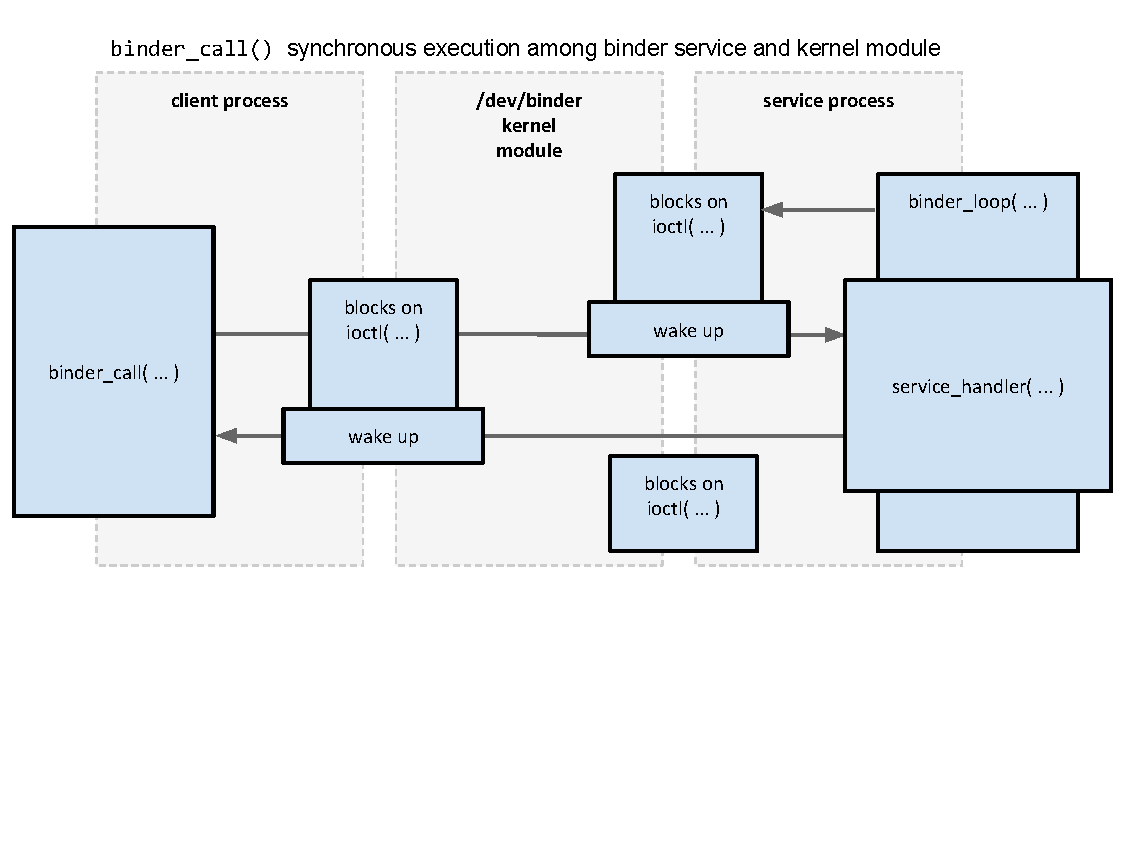
\includegraphics[width=\textwidth]{drawings/binder_call.pdf}
\caption{binder\_call synchronous IPC execution among binder service and kernel module}
\label{fig:binder_call}
\end{figure}

\subsubsection{binder\_io with objects and file descriptors}
An essential feature of binder is the ability to write binder objects and file descriptors as arguments into (or in replies from) RPCs. A process can obtain a handle to a remote object this way, and can invoking a RPC on the remote object as a callback for example. Both primitive types and objects are written into the binder\_io byte-array. A handle to an object is an descriptor that is tracked by the kernel module, and the Binder driver takes care of rewriting the structure type and data as it moves between processes~\cite{BinderSourceComment}. This level of understanding of BKM is sufficient in detail for the scope of this paper. Documentation on internals of binder is sparse. The following references~\cite{BinderLinuxFoundation,BinderMastersThesis} provide a useful resource, but the real reference to Binder is in code--its implementation in Android.

\subsection{Binder within the Android Runtime}
The Android Runtime has several layers of abstractions built on top of the basic BKM. All these layers eventually result in calls either to the lowest-level C API which we have just covered or directly operate on the kernel driver. The main difference is that the C++ and Java APIs are object-oriented (OO), defining an IBinder interface which binder services implement. transact(...) is the method to perform generic operations to implement RPC. It very much resembles the low-level C API's binder\_call(...) function. The OO implementation also encapsulates binder\_io structures as Parcel objects.

\begin{snippet}[label=snip:IBinder]
interface IBinder {
  // Get the canonical name of the interface supported by this binder.
  String getInterfaceDescriptor();
  boolean transact(int code, Parcel data, Parcel reply, int flags);
  void linkToDeath(DeathRecipient recipient, int flags);
  boolean unlinkToDeath(DeathRecipient recipient, int flags);
}
\end{snippet}

The OO Binder follows the Proxy Pattern~\cite{ProxyPattern}. BBinder is a class that is instantiated as the real implementation of the service. It calls the equivalent of binder\_loop and accepts transaction requests. Then there is BpBinder which is a proxy class that is insntantiated with a remote handle to an active BBinder service. Analogously, there is a Java implementation that has a mirror IBinder java interface~\ref{snip:IBinder}, defining Binder and BinderProxy classes which encapsulate the native BBinder and BpBinder classes, respectively, via JNI.
%\begin{figure*}
%\centering
%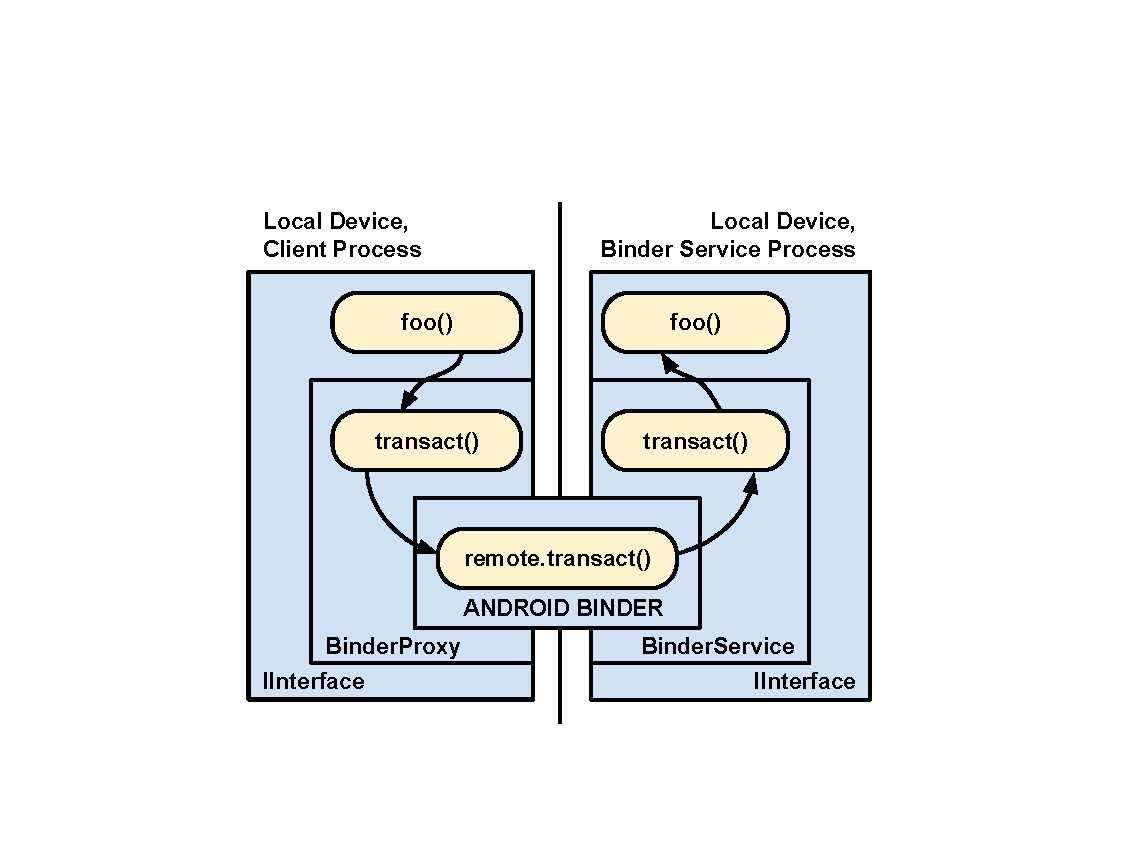
\includegraphics[width=0.3\textwidth]{drawings/proxy_pattern.pdf}
%\end{figure*}

An invokation of BpBinder.transact() simply invokes a binder\_call to its remote handle, and via binder invokes the BBinder.transact() method on the remote process. A service is implemented on top of this structure, by extending the two classes and following a convention to implement RPC via calls to transact(). For instance, a FooBarService is implemented by associating each method with an ID, passed in as the code argument into transact().

\begin{snippet}
class BpFooBarService : public BpBinder {
  void foo(int a, int b) { /* ... */ transact(1, encoded_args, ...); }
  void bar(string c) { /* ... */ transact(2, encoded_args, ...); }
  /* transact() calls remote binder, waits, and returns reply. */
}
class BnFooBarService : public BnBinder {
  void foo(int a, int b) { /* Do something useful */ }
  void bar(string c) { /* Another useful fucntion */ }
  void transact(code, msg, reply, flags) {
    switch(code) {
      case 1: /* decode args... */ foo(args); break;
      case 2: /* decode args... */ bar(args); break;
}}}
\end{snippet}

The creation of binder RPC involves boilerplate code. To make this more convenient, the Android SDK defines a domain-specific language named AIDL to specify interfaces for binder services in a language similar to the language for specifying Java interfaces. The AIDL compiler generate Stub and Proxy classses that implement the specified interface and encapsulate Binder and BinderProxy objects, respectively. A developer simply extends the Stub class, providing an implementation for each service method (like foo() and bar() above). The generated classes do all the necessary work to marshall and unmarshall arguments as Parcels and invoke the appropriate method on the actual service object. For instance, here is the AIDL definition of the FooBarService.

\begin{snippet}
interface FooBarService { void foo(int a, int b); void bar(String c); }
\end{snippet}

A binder object implementing a specified service interface can be created simply by extending the Stub class, providing an implementation for service methods.

\begin{snippet}
IBinder localBinder = new FooBarService.Stub() { void foo(...) { ... }
                                                 void bar(...) { ... } };
\end{snippet}

\subsection{Accessing Binder Services}
The Android Runtime provides pathways for components to communicate binder objects between themselves. For instance, Android apps can declare a Service component that other components, like GUI Activity components, can bind to.

\begin{snippet}
class FooBarAndroidService extends Service {
  public void onBind() { return new FooBarService.Stub() { ... }; }
}

class FooBarClient extends Activity {
  public void onStart() { bindService(/* name of the service */,
                                      /* callback on connected */ this);
  }
  public void onServiceConnected(
    Context context, IBinder binder) {
    // The binder here is a BinderProxy, not the original Binder object.
    FooBarService.asInterface(binder).foo(1, 3);  // invokes RPC.
  }
}
\end{snippet}

As we see above, retrieving a non-system service is just a simple asynchronous operation from the perspective of the app developer. However, there are a few core services of the Android Runtime that come into play to make it happen. The process is visualized in figure~\ref{fig:BindService} and detailed below.

\begin{figure}[h]
\centering
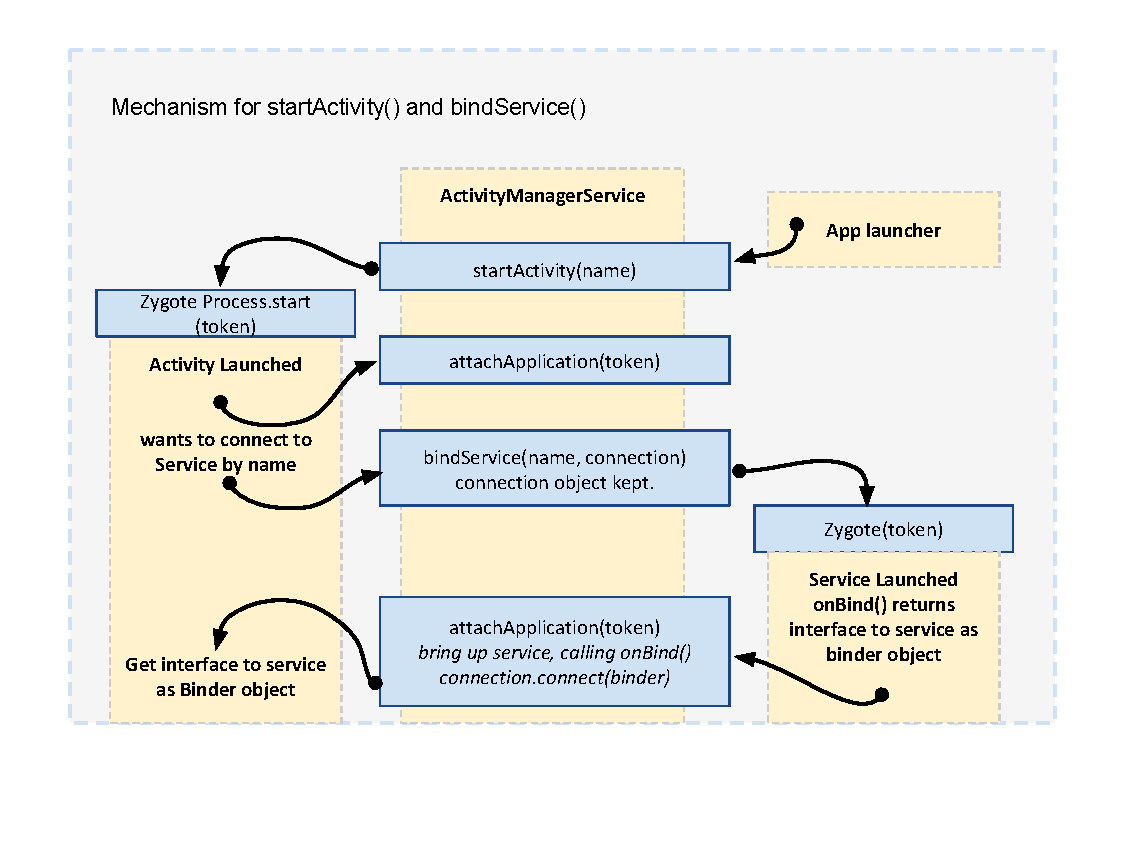
\includegraphics[width=0.85\textwidth]{drawings/bindService.pdf}
\caption{Android Runtime and Components Interaction after a bindService() RPC}
\label{fig:BindService}
\end{figure}

bindService(...) is invoked with a callback binder object--the ServiceConnection. Once the requested service is up, the ServiceConnection callback is invoked asynchronously with the requested binder service as an IBinder object. The ActivityManager works together with other essential system services to bring up and connect to the specified service component. The PackageManager, which tracks all installed components on the system, validates that the requested service component exists and checks that the caller has permissions to connect to it. If the requested service resides in a separate java package, a low-level component known as Zygote brings up the service as a separate process. When the service is up, it attaches to the ActivityManager via RPC. Afterwards, ActivityManager retrieves the binder service provided by the service component as an IBinder object, and passes it on the caller by invoking the ServiceConnection callback. There are quite a few RPCs involved in this procedure!

\subsubsection{Accessing Android System Services}
bindService(...) cannot be used for everything. For instance, in the course of binding to a service, the ActivityManager brings up the service first and waits for it to attach. The service cannot use bindService() to get a reference to the ActivityManager, as that is a circular dependence. Instead core system services like ActivityManager are all available through the ServiceManager--the binder kernel module's default context manager. It is straightforward to obtain a reference to the ServiceManager from any process or thread (i.e. make binder\_call with target=(void*)0). So it follows that it is always possible to retrieve IBinder references to any currently active service published to the ServiceManager.

The direct method using binder\_call() to communicate with ServiceManager (as in Example~\ref{snip:binder_call}) is not strictly necessary. Rather, ServiceManager has an OO Binder interface, this interface is provided in the Appendix~\ref{app:ServiceManager}. 

\section{System Services: Provided Over the Network?}
\label{sec:SystemServices}
Before going into the design and implementation of Sigma, it is useful to understand first what all system services that are offered via binder. This will serve as motivation to figure which feature of binder we will have to support in Sigma. In particular, we want to answer: which services are useful for remote devices to access? And which cannot be accessed (or don't make any sense to provide access to)?  To start, it is reasonable to expose ServiceManager since it is an entry-point into all other system services. There are dozens of system services, four are covered here.

\subsection{LocationManager: location updates via binder callback and PendingIntent}
It is most natural to expose system services that are standalone and isolated in a sense. A good example is the LocationManager which ``allows applications to obtain periodic updates of the device's geographical location, or to fire an application-specific Intent when the device enters the proximity of a given geographical location.~\cite{LocationManagerDocs}'' The location manager operates as a standalone source of location updates. Here are 2 methods of the LocationManager that we look into further.

\begin{snippet}
interface ILocationManager {
  void requestLocationUpdates(
      in LocationRequest request,
      in ILocationListener listener,
      in PendingIntent intent,
      String packageName);
  void removeUpdates(
      in ILocationListener listener,
      in PendingIntent intent,
      String packageName);
  // ... among other methods
}
\end{snippet}

\begin{snippet}
oneway interface ILocationListener {
    void onLocationChanged(in Location location);
    // ... among other callback methods
}
\end{snippet}

The main requestLocationUpdates() method requires the client to provide either a ILocationListener binder callback or PendingIntent callback. If the former callback is initialized locally and passed in as a binder argument. Then the LocationManager holds a BinderProxy (a weak reference) to it the callback object, and invokes the .onLocationChanged() RPC periodically with location updates. The provided caller application has to keep a the callback object alive and itself remain active for callbacks to work correctly.

The latter PendingIntent callback is also implemented via binder. However the mechanism is provided by the Android Runtime. A PendingIntent is owned by the Android Runtime, and the caller first obtains a reference to it from the central ActivityManagerService. A PendingIntent is constructed with the address of a recipient (callback) android component to which future messages are delivered. Working as a callback mechanism, the PendingIntent is usually initialized with the caller's own component address. When provided as argument to the requestLocationUpdates() method, the LocationManager later can invoke the PendingIntent.send() RPC with location updates as contained data. This RPC goes to the Android Runtime (the owner of the PendingIntent), which then via another RPC routes the message to the recipient component. Though the PendingIntent mechanism is inherently more complex, the advantage is that the Android Runtime takes case to brings up the recipient component in case it is not already up. This way an app can register a PendingIntent callback and not have the burden of being active to receive callbacks.

\begin{snippet}
interface IIntentSender {
  int send(
    /* The message */
    int code, in Intent intent,
    /* Address of recipient */
    String resolvedType,
    /* Send finished callback */
    IIntentReceiver finishedReceiver,
    ...);
}
\end{snippet}

\begin{snippet}
oneway interface IIntentReceiver {
  void performReceive(
      in Intent intent, int resultCode,
      ...);
}
\end{snippet}

PendingIntent.send() is implemented in non-blocking fashion. Hidden from view, the PendingIntent is constructed with reference to a IIntentSender binder service object which is owned by (and runs within) the ActivityManager. An additional IIntentReceiver callback can be passed in with each invokation of .send() to be notified once the send operation is complete. The LocationManager uses this send and together with a finishedReceiver callback to hold what's known as a WakeLock--an Android Runtime feature used to prevent the device from entering sleep mode. Without the WakeLock, messages would be stuck in-flight and delivered only when the device wakes up from sleep.

Both direct binder object callbacks and PendingIntent callbacks should be supported by Sigma. PendingIntent callbacks are of particular interest since they can be used in the design of ``push'' services~\cite{PushTechnology}. A client can register a PendingIntent with a service provided by a remote device. Subsequently the local app can receive messages without the need to be always active. Of course, the Sigma network stack in charge of receiving remote binder messages and the service on the remote device itself have to be always active for this to work.

\subsection{SensorManager: sensor events via unix domain sockets}
The SensorManager is another good candidate to allow access to remote devices. It is a standalone source of sensor data streams. Recently, sensors services have evolved to to provide the user's activity state--e.g. categories like walking or driving. We image the future of sensor services will include an variety of contextual inferences.

Also, SensorEvents are sent via a BitTube--an OO abstraction on top of unix domain sockets. So this is a system service that uses binder to setup a socket connection between two processes. Subsequent communication of sensor events is sent as messages over the socket. If we are to expose SensorManager over the network, we need to the ability to send file descriptors (and importantly: to support IO operations on those file descriptors) over the network as well.

\begin{snippet}
class ISensorServer : public IInterface {
public:
    Vector<Sensor> getSensorList() = 0;
    sp<ISensorEventConnection>
      createSensorEventConnection()
    // ... among other methods
};
\end{snippet}

\begin{snippet}
class ISensorEventConnection : public IInterface {
public:
    sp<BitTube> getSensorChannel()
    status_t enableDisable(int handle, bool enabled)
    status_t setEventRate(int handle, nsecs_t ns)
};
\end{snippet}

\subsection{AlarmManager: not very useful over the network}
There are some services which don't make too much sense to expose. For instance, the AlarmManager is ``intended for cases where you want to have your application code run at a specific time, even if your application is not currently running.'' There is no need to access a remote device's alarm manager as it provides no useful data or service more than the local instance of AlarmManager.

\subsection{ActivityManager: difficult to expose over network without extensive refactoring}
Services that are not standalone or are coupled to the local context of Android applications are difficult to directly expose over the network. This is because the operation of such services depends on records that are local to the device. For instance, ActivityManager is a crucial system service that is in charge of managing all live components running on the Android device. It provides useful operations such as bindService().  However, it is not so straightforward to invoke bindService() on a remote handle to ActivityManager since the call depends ActivityManager's records about the calling process that only the ActivityManager on the caller device knows about.

\subsection{A caveat with Android Permissions}
A complication, particularly when dealing with system services, is that many of them require permission to access. That is, local apps declare permission to use a service, and the PackageManager grants such permission at install time. It is not trivial to extend the Android permissions system to allow for remote binder objects. As such Sigma as it is implemented disregards Android permissions, allowing remote devices access to all services running on a device. A thorough treatment of the permissions framework and its support in Sigma is a left for future work. A discussion on this topic is found at the end of the paper in Sections~\ref{sec:DealingWithAndroidPermissions} and ~\ref{sec:NextSteps}.

\section{Sigma: Design and Implementation}
\label{sec:Sigma}
\begin{figure}[h]
\centering
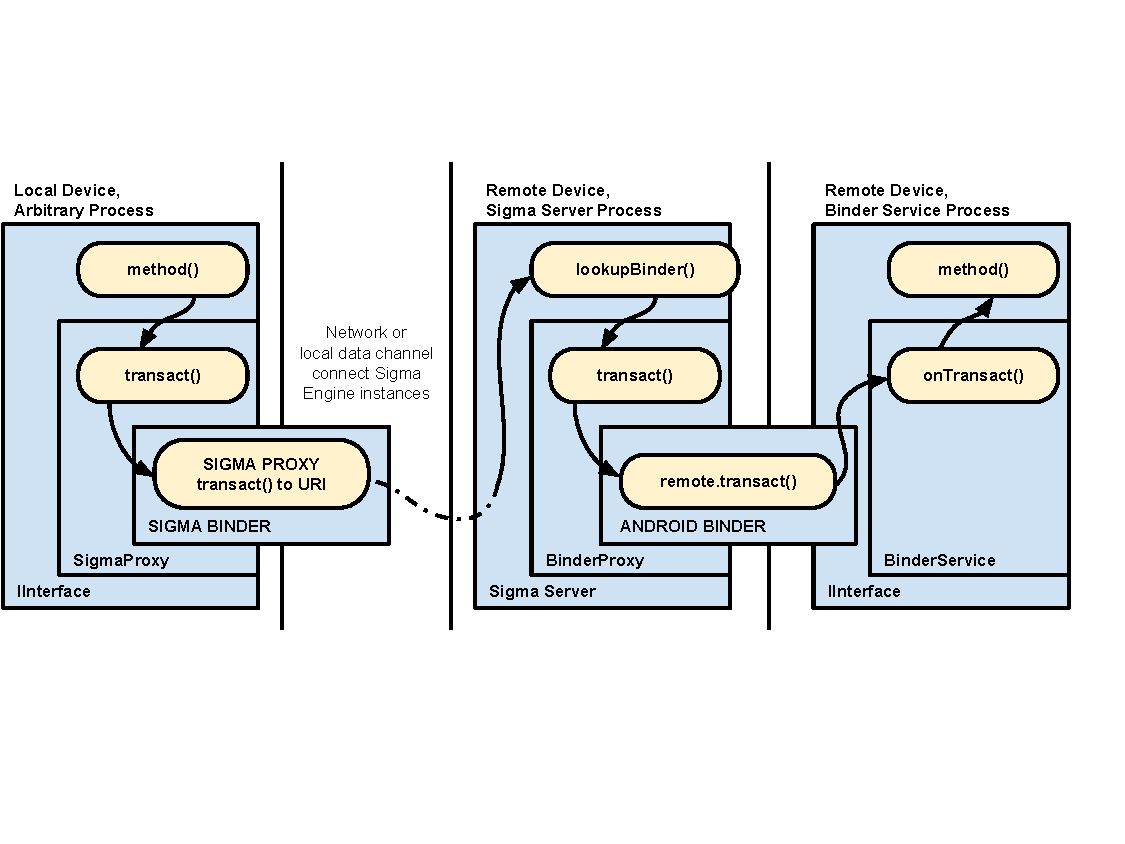
\includegraphics[width=0.8\textwidth]{drawings/sigma_proxy_pattern.pdf}
\caption{Sigma as a Chained version of the Proxy Pattern}
\label{fig:SigmaChainProxy}
\end{figure}
The goal of Sigma is to essentially to follow the Proxy Pattern of binder services one hop out--tunneling binder transactions over the network, see figure~\ref{fig:SigmaChainProxy}. The design of Sigma should minimally modify the Android Runtime, while supporting both native and Java-based binder services. And, perhaps most important: Sigma should support binder's powerful feature to allow the passing of binder objects and file descriptors as arguments in a remote RPC call. This last issue will be addressed in the second-part of this section.

\subsection{Proxy Pattern over the Network}

Consider a network consisting of two Android devices, and that there is a pre-established data channel between them. Each device runs a Sigma Engine instance which has server-like and client-like functions. Its function viewed as a server is to associate a URI to local binder services, and subsequently accept binder transaction requests made to a URI--performing the binder transaction on the associated local binder. Its core function as a client is to allow the retrieval of remote binder objects (retrieved as a URI) and implement the Proxy Pattern, passing on the Proxy IBinder to local services. Subsequent binder transactions invoked on the proxy object forward the transaction over the network to the associated URI.

Binder services are often implemented in Java with AIDL-specified interfaces. But not always. Binder services can also be hand-made (in c, c++, or java) following any arbitrary convention for doing RPC. A binder service simply has to use the BKM in some way to qualify as one. Fortunately, all Android binder services follow the IBinder interface. So the goal of Sigma is to proxy all methods of the IBinder interface. Also, fortunately, the Java and C++ versions of IBinder specify identical interfaces that are compatible with one another. In fact the Java implementation is really a JNI-based wrapper of the C++ version. Native services can be first proxied into a Java BinderProxy.

Sigma Engine needs a networking stack to work with. It makes most sense to implement this part at the Java level--using the features of the Java Android Runtime (and convenience of the SDK) to full benefit. Networking libraries are readily available for Android as pure Java libraries. Moreoever, this way Sigma can be packaged as any other third-party app. Distributed and installed through the app store.

\subsection{Necessary Modifications to the Android Runtime}
\label{sec:AndroidRuntimeModifications}
Unfortunately, there are a few obstacles to an implementation in the default Android Runtime. The implementation of Java Binder and BinderProxy does not expose native handles to BBinder and BpBinder. In addition, there is no method to create Java Binder objects out of native handles. So if we are to implement Sigma in pure Java as it is, we have no hope of creating proxy interfaces to native binder services. An example of such a service is the SensorService. The remedy is to modify the Android Runtime. The following are signatures of added methods that do the job of converting from native binder to Java binder and vica-versa.

\begin{snippet}
class BinderInternal {
  // ...
  native IBinder binderForNativeHandle(int handle);
  native int nativeHandleForBinder(IBinder binder);
}
\end{snippet}

Binder transactions operate on binder\_io arguments which may contain objects and file descriptors. The BKM specially rewrites these objects, and so the binder\_io data structure has an offsets array containing information about where each object or file descriptor is in the data array. It follows that Sigma, in proxying binder transactions, also has to specially manage such arguments--these details we will leave for the next section. As a first requirement though, we need to access the offsets array from Java--where Sigma is implemented. Unfortunately, the Java and C++ Parcel objects which encapsulate the binder\_io data structure prevents access to this very important offsets array. Without it, we cannot know where and how may objects are in contained in the Parcel. Because this is an essential requirement, and we resort to modify or add methods to the Android Runtime to allow access.

\begin{snippet}
class Parcel {
  public static byte[] marshall();
  public static void unmarshall(
      byte[] data, int offest, int length);

  public static int[] getObjectPositions();
}
\end{snippet}

The marshall() and unmarshall() methods are already present in the default Parcel implementation, but it cannot handle Parcels that contain objects elements--we have fixed it to not care about that. The getObjectPositions() method is new it simply provides access to the underlying offsets array.

The source code to the modified Android Runtime is available online, see Appendix~\ref{app:SourceCode}. It is available as a patch for a particular version (4.2.2) of Android, but these changes should be compatible with the vast majority of Android versions with only minor modifications. The rest of the paper assumes a that we operate on the modified runtime.

\begin{snippet}
parcel.setDataPosition(offset);
IBinder binder = parcel.readStrongBinder();
\end{snippet}

\subsection{Design of the Sigma Message-based Protocol}
Having established that all the necessary pieces are accessible from the modified Java Android Runtime, we will now detail the design and implementation of the Sigma Engine which is a seen as protocol for retrieving binder objects as URIs and performing binder transactions on it.

Assuming we have established a data channel between two devices, the first decision is to chose a structured format for communication over the channel. There is a lightweight implementation of Google's protobuf language for serialized objects called Wire~\cite{Wire,IntroWire}. It is a open source library created specifically for Android by the mobile app company Square. The protocol between Sigma Engines is modeled via transactions, the exchange of as Wire messages. Each transaction is composed of SRequest followed by SResponse. Figure~\ref{fig:GenericSigmaTransaction} contains pseudo-code of the protobuf implementing the generic transaction.

\begin{figure}[h!]
\centering
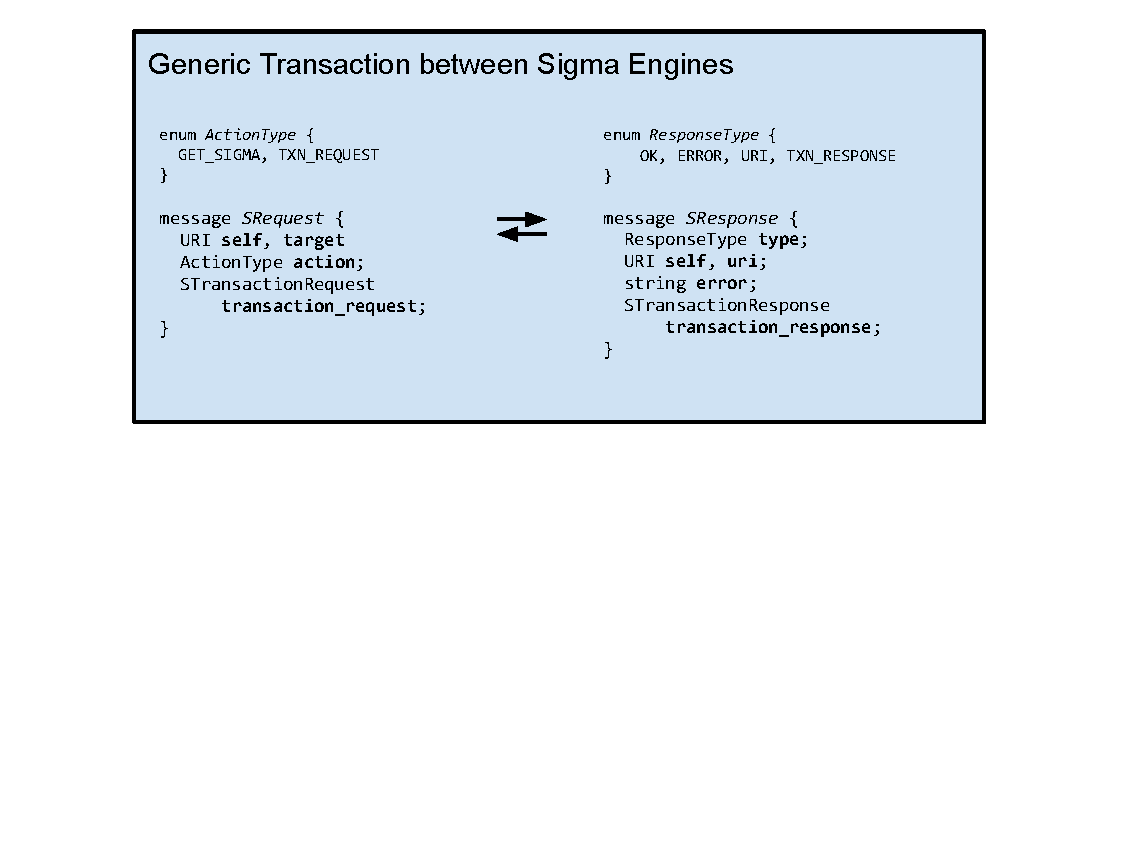
\includegraphics[width=0.8\textwidth]{drawings/WireTransaction.pdf}
\caption{Generic Sigma Transaction}
\label{fig:GenericSigmaTransaction}
\end{figure}

The URI is a Wire message (see Figure~\ref{fig:WireURI}) that contains always contains the network information about a Sigma Engine. This is known as a BASE URI. For instance, an HTTP-based Sigma Engine has a URI with the host and port fields set. A URI can also reference a remote object. A BINDER URI is a BASE URI with additional fields like the an id of the referent binder and its interface descriptor.

\begin{figure}[h!]
\centering
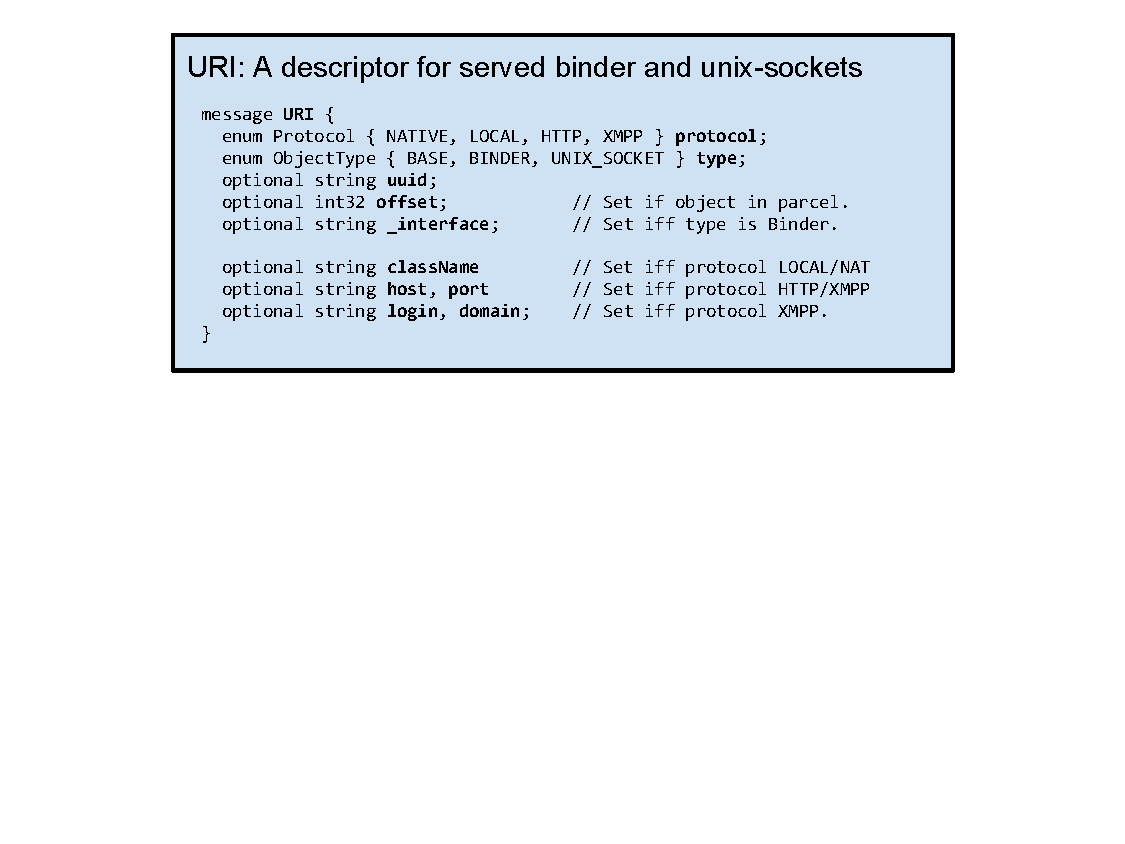
\includegraphics[width=0.8\textwidth]{drawings/WireURI.pdf}
\caption{Wire URI message}
\label{fig:WireURI}
\end{figure}

A proxy binder object is initialized with the received BINDER URI as target. A transaction invoked on the proxy causes a network transaction to occur. This starts with an SRequest sent to the remote Sigma Engine. The remote Sigma Engine performs the transaction and returns a SResponse containing the reply. The transaction request and response both contain parcels encoded as SParcel, where the data array is first Base64-encoded to a string. These Wire messages format are in Figure~\ref{fig:GenericSigmaBinderTransaction}.

\begin{figure}[h!]
\centering
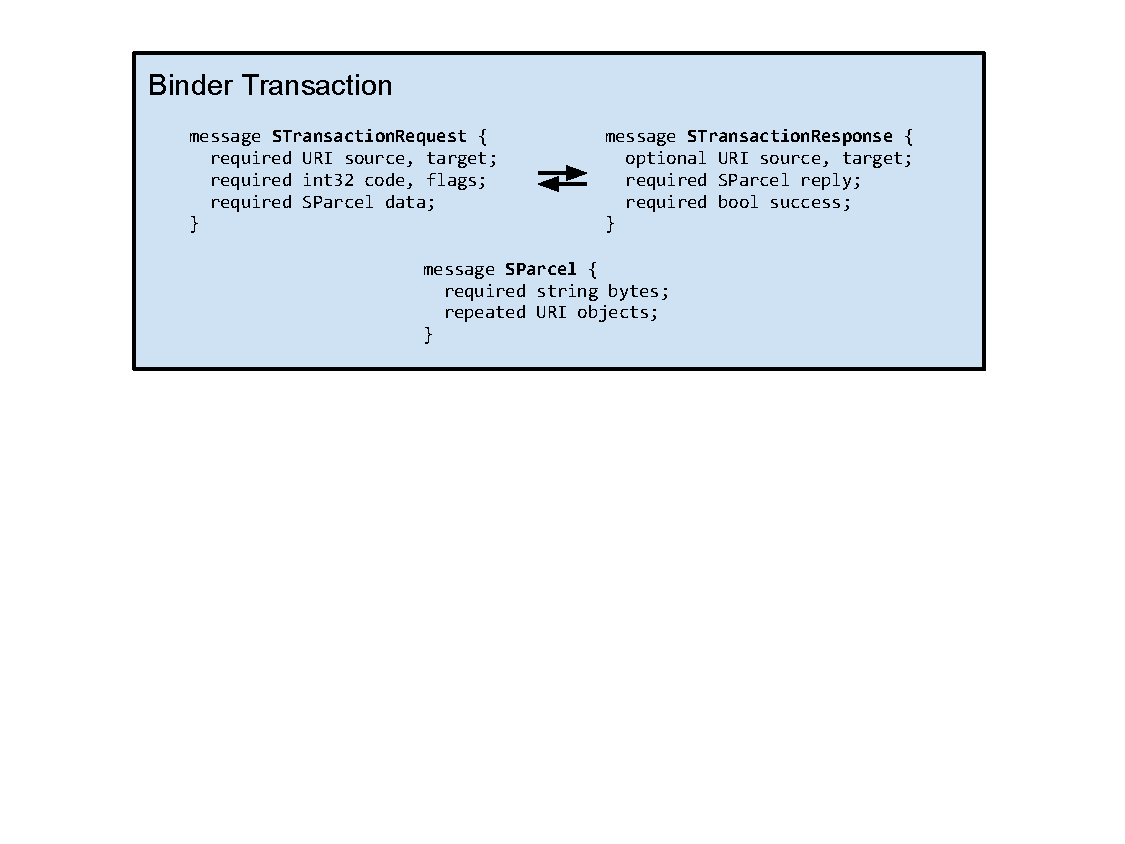
\includegraphics[width=0.8\textwidth]{drawings/WireBinderTransaction.pdf}
\caption{A Generic Sigma Binder Transaction}
\label{fig:GenericSigmaBinderTransaction}
\end{figure}

Another detail is reference-counting. We do not want Sigma Engine managed binder objects to remain dangling. Fortunately, Binder objects are reference-counted by the Binder framework. As long as we take care to keep only weak references to created Binder objects, the Binders will be automatically finalized when no valid references to it remain. When this happens, we send a clean-up message to remote Proxies ensuring that there are no dangling references (i.e. to finalized BINDER URIs).

\subsection{Tunneling Binder Descriptors}
As we know, binder objects can be contained in the Parcel passed into a binder transaction. When we encounter this situation, the Sigma Engine takes ownership of the contained binder object and assigns to it an ID. This ID is transformed into a BINDER URI (taking the local Sigma Engine's BASE URI and adding on the ID of the managed binder object). In this way, Parcels containing binder objects are encoded as SParcel messages with containing an array of corresponding URIs in the objects field.

Conversely, a Sigma Engine can receive remote binder transaction requests with SParcels that have a non-empty array of BINDER URI objects. In this situation, a local Binder is created and managed by Sigma Engine. The local binder is a special Proxy that forwards local transactions made on it to the BINDER URI target that it was initialized with.

\begin{figure}[h]
\centering
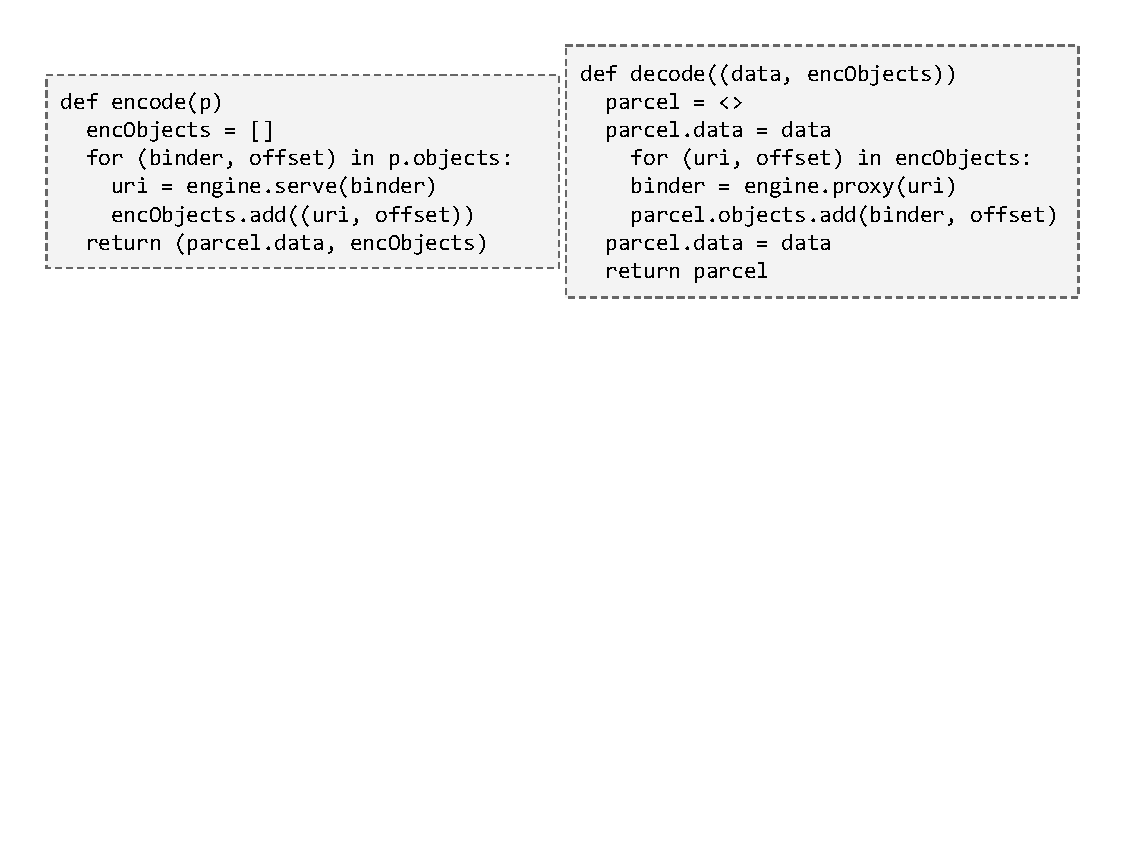
\includegraphics[width=0.8\textwidth]{drawings/encodeObjects.pdf}
\end{figure}

\subsection{Tunneling File Descriptors over Network}
File descriptors in Parcels are handled analogously to binder objects. However, in Unix-like systems, file descriptors can refer to any Unix file type named in a file system. As well as regular files, this includes directories, block and character devices (also called ``special files''), Unix domain sockets, and named pipes. File descriptors can also refer to other objects that do not normally exist in the file system, such as anonymous pipes and network sockets~\cite{UnixDomainSocket}.

Although it is theoretically possible to handle each type file descriptor (like the command-line utility nc that exposes each over a socket), each type has to be treated separately since each type has a specific set of supported IO operations. We only want to demonstrate as a proof-of-concept that we can handle file descriptors by focusing on a single type: the Unix domain socket. These special sockets are used to communicate sensor events in SensorManager, and used elsewhere in GUI-related Android services, so there is a valid use case. Such file descriptors are created via socketpair() with the protocol SOCK\_SEQPACKET, and provide sequenced, reliable, bidirectional, connection-mode transmission paths for records. A record can be sent using one or more output operations and received using one or more input operations, but a single operation never transfers part of more than one record~\cite{SocketManPage}. Fortunately, we need to support only a small set of operations: send() and recv(). Also the remote end needs to know when the socket is no longer valid or is otherwise closed so that resources can be cleaned up.

Unlike a binder object where requests go only from proxy to server, the socket is bidirectional. So a when Sigma Engine receives a local transaction with a unix domain socket in the Parcel, it takes ownership of the file descriptor and creates a corresponding a UNIX\_DOMAIN\_SOCKET URI that is encoded into the SParcel.

At the the remote end, receiving SParcels with UNIX\_DOMAIN\_SOCKET URIs creates a local unix domain socket which is written into the Parcel in completing the binder transaction.

\begin{figure}[h]
\centering
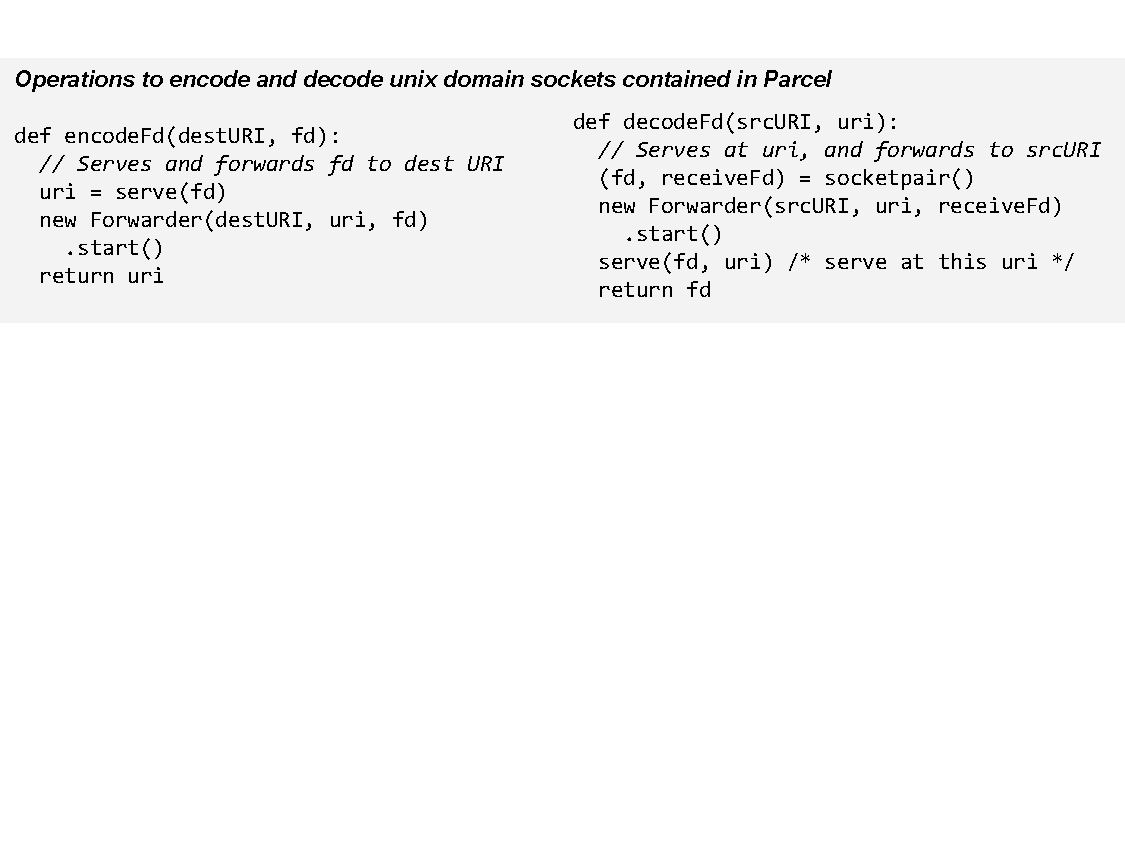
\includegraphics[width=0.8\textwidth]{drawings/encodeFds.pdf}
\end{figure}

Creating and exchanging the URI for the file descriptor is only the first step. IO Operations need to be forwarded. A Forwarder object is initialized to poll the file descriptor and on receiving data, forwards the data over the network addressed to the appropriate UNIX\_DOMAIN\_SOCKET URI. On the other side, socket data received at a UNIX\_DOMAIN\_SOCKET URI is forwarded locally to the local managed file descriptor.
\begin{figure}[h]
\centering
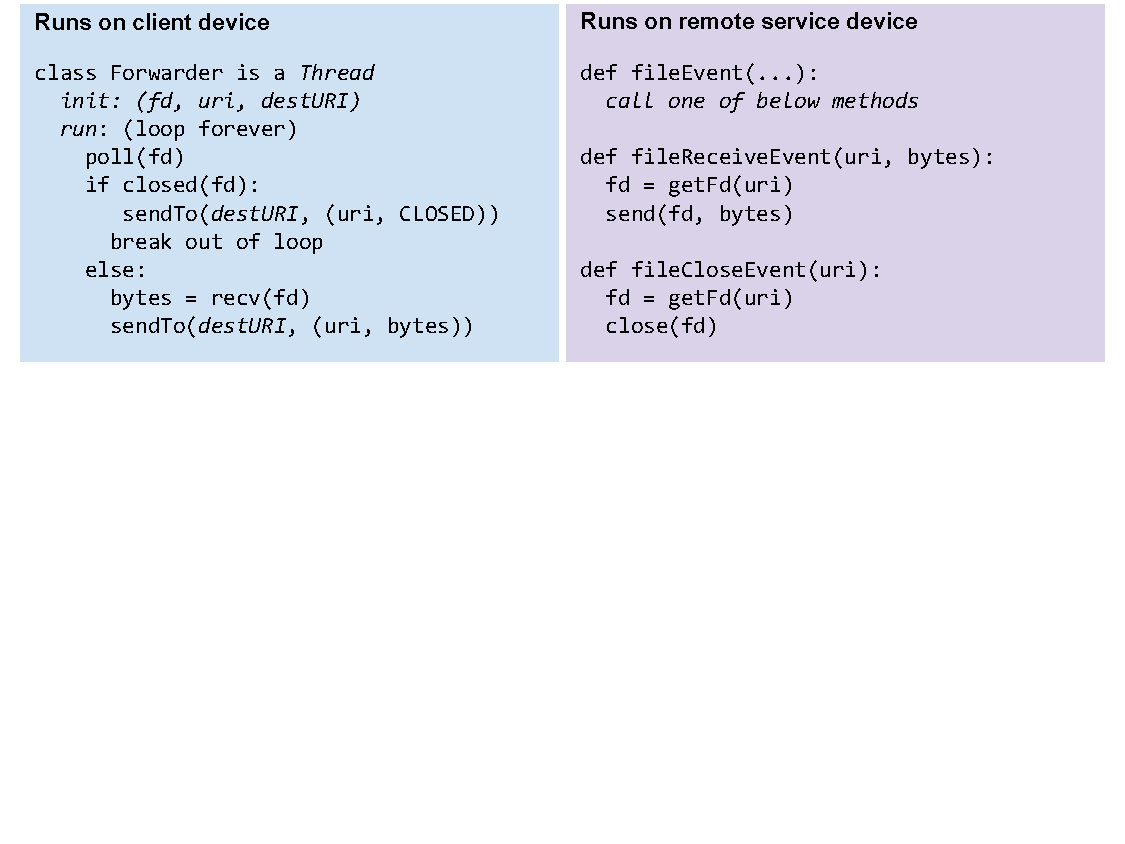
\includegraphics[width=0.8\textwidth]{drawings/forwardFds.pdf}
\end{figure}

\subsection{Choice and Implementation of a Networking Stack}
Sigma is first a protocol and then an implementation. As a protocol, it is agnostic to the network connection, assuming only that a reliable underlying data channel is available for atomically sending and receiving messages. For instance, one version of Sigma is implemented locally using Android Binder itself as a data channel. This is useful for testing as we can run two instances of Sigma engine on the same device. To evaluate Sigma between Android devices, we have a gamut of networking technologies to choose from. We choose HTTP- and XMPP- based channel to test evaluate the design and measure performance.

\subsubsection{Sigma Engine over HTTP}
In this mode, each device brings up a HTTP server listening on a pre-determined port. Clients communicate to another device by performing an HTTP POST request to another device's HTTP server. The client needs to know the IP or hostname of the server and the server must be accessible over the network.

\subsubsection{Sigma Engine over XMPP}
In this mode, each device login with distinct handle to a mutually accessible XMPP server. XMPP is a popular protocol for real-time collaboration--messaging and chat. The data channel is through chat threads with other active handles. Each thread serves one transaction, similar to what is available in one HTTP POST request. Chat threads are limited to one request and to one reply. Future (or parallel) transactions occur on separate threads.

\subsubsection{Encoding Sigma (Wire) Messages, Examples}
The Sigma Engine creates Wire messages for each transaction. These can be printed to human-readable format. For instance, here is a URI to an XMPP-based SigmaEngine.

\begin{snippet}
URI{_interface=com.example.BinderSigma.samples.chat.ICommentReceiver,
domain=quark, login=rr, protocol=XMPP, type=BINDER,
uuid=c2f980b5-ae50-4f7e-9559-438abc49508f}
\end{snippet}

Such Wire messages are compactly serialized into byte arrays. Over HTTP, the byte array is sent directly via a POST request as a byte-array entity. Over XMPP, the byte array is first made into a Base64-encoded string and then sent as a chat message. Below is an example of a SRequest sent as an XMPP chat message (note: the SRequest is serialized then Base64-encoded)

\begin{snippet}
<message type="chat" id="30e5a4c7-b0d7-4d11-bd2c-14abf4ff1ce0"
        to="kk@quark" from="rr@quark/Smack" >
        <body> <!-- Base-64 encoded string --> </body>
        <thread>877a1f <!-- id of transaction --> </thread>
        </message>
\end{snippet}

The Appendix~\ref{app:WireExchange} and ~\ref{app:WireExchangeRecursive} contains a section with examples of actual Wire messages exchanged in implementing the example at the beginning of this sections.

\subsection{Sigma as a binder service itself}
The Sigma Engine is implemented as an Android service component. It is brought up with a BASE URI that serves as the Sigma Engine's identity going forward. There are separate services for each different implementation (i.e. LOCAL, HTTP, XMPP). Bringing it up any Sigma Engine service component and binding to it returns a remarkably simple binder service interface. This is the interface which can be used by app developers to get remote services as IBinder objects.

\begin{snippet}
interface ISigmaManager {
    URI getBaseURI();
    ISigmaManager getRemoteManager(in URI targetBaseURI);
    IBinder getServiceManager();
    /* synchronous version of bindService(Intent...) */
    IBinder getService(in Intent intent);
}
\end{snippet}

Consider an example. Assume that there is are two distinct sigma engine instances, $\Sigma$A and $\Sigma$B, running on two devices, named A and B respectively. An app can access its own local Sigma Engine instance and make use of the provided ISigmaManager service. The following pseudo-code walks through the steps taken by an app running on device A to access a remote service from installed on device B. It is assumed $\Sigma$B is already up and running, listening for connections.

\begin{snippet}
uriB = /* given the URI $\Sigma$B is already known */
sigmaManA = connectToLocalSigmaEngine($\Sigma$A)
sigmaManB = sigmaA.getRemoteManager(uriB)
remoteBinder = sigmaManB.getService("name.of.remote.service");
remoteBinder.foo() /* Invoke remote binder RPC via Sigma Proxy */
\end{snippet}

To get a sense of the interaction between the processes on the two devices, figure~\ref{fig:SigmaInteraction} is a useful visualization.

\begin{figure}[h]
\centering
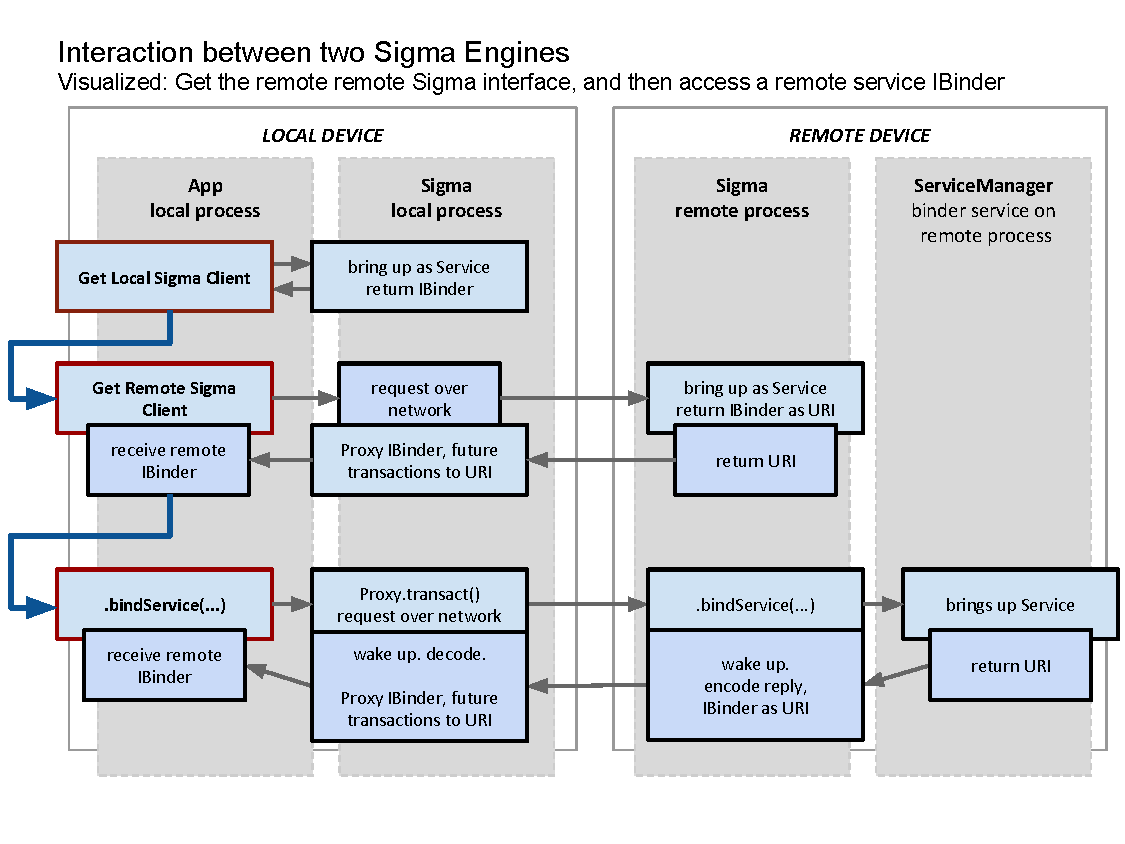
\includegraphics[width=0.8\textwidth]{drawings/SigmaEngineInteraction.pdf}
\caption{Interaction between Sigma Engines in obtaining a refernce to a remote service.}
\label{fig:SigmaInteraction}
\end{figure}

\subsection{Accessing remote system services}
All system services are published to the ServiceManager. A client app can access the remot service manager by performing the .getServiceManager() RPC on a remote ISigmaManager. However, the remote service interface is usually not the interface used by client apps. Often the remote interface is wrapped up in local client object that provides the final service to clients. To alleviate this issue, Sigma provides a convenient RemoteContext class that is constructed with reference to a remote ServiceManager. It provides a getSystemService(name) method that implements code to retrieve remote system services and wraps them up in a client object that is more usable.

As a proof-of-concept we have implemented the retrieval of two remote services--the LocationManager and SensorManager. Many services are easily wrapped in local client objects. The local LocationManger client is straightforward to construct using reflection from the internal ILocationManager service. However, SensorService (the intenral binder service providing sensor events) has a local client with parts implemented in C++ and other parts in Java (via JNI). This is not usually a issue, but the SensorManager is hardcoded to retrieve only the local SensorService! So it is impossible via reflection or other hacks to construct a SensorManager client with a remote SensorService handle. To enable this, we had to modify the Android runtime--the source code is available online, the link is found in Appendix~\ref{app:SourceCode}.

\section{Performance Evaluation}
\label{sec:Performance}
It is useful to know the CPU cost and latency to establish a proxy to a remote binder service and then the cost to make RPCs on that Proxy. Overhead is expected due to the additional IPC within each device (there is communication from apps and services to the Sigma Engine). There is also the cost of encoding/decoding parcels during binder transactions, of creating requests and response messages, and naturally there is some cost to have network stack perform IO. We first describe some simple test binder services and then present the execution timing for invoking RPCs on these test services.

\subsection{Testing Simple Binder Services}
As a first test, consider a trivial binder service: a random number server. The interface is below.

\begin{snippet}
class RandomServer extends IRandomServer.Stub() {
  int getRandom() {
    return (new Random()).nextInt(); }
}
\end{snippet}

As a second test, consider a binder service that accepts binder object arguments. In particular, using this feature it is possible to specify a callback object that invokes a binder transaction back to the local device. Taking it one step further, recursion can occur back-and-forth as a series of binder calls between the two devices. The following binder service called PingPongService implements such a test. A local instance is passed in to invoke a method on the remote instance, starting in a recursive case like: remote.ping(local, 10). This causes a cascade of recursive calls, each counting down the number argument.

\begin{snippet}
class PingPongService extends
    IPingPongService.Stub() {
  void ping(IPingPongService other, int count) {
    if (count > 0) other.pong(this, count - 1);
  }
  void pong(IPingPongService other, int count) {
    if (count > 0) other.ping(this, count - 1);
  }
}
\end{snippet}

\subsection{Performance Measurements}
Here is the result of timing various RPCs, from above. These are timed for 3 prototype implementations each using a different type of data channels for communication.

\begin{figure}[h]
\centering
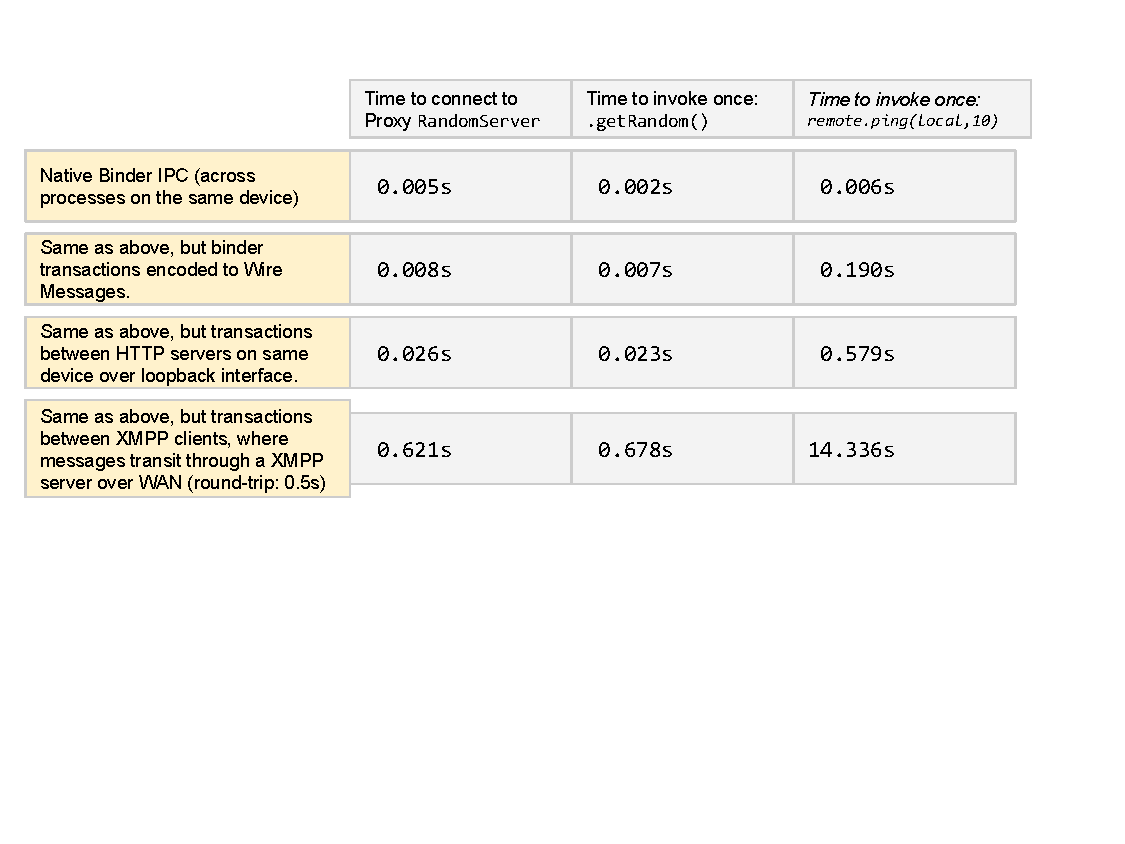
\includegraphics[width=0.85\textwidth]{drawings/Performance.pdf}
\end{figure}

As is apparent, it is 2x-3x as expensive to perform a binder call over a proxy that encodes messages than it is to make a straight, native binder call. However, the recursive PingPong test is quite expensive since each recursive call is a new binder transaction with another round of encoding and decoding, with added network overhead.

\subsection{Testing Performance with System Services}

The following assumes knowledge of the respective system services, a overview of which is provided at the beginning sections of the paper.

\subsubsection{Remote Location Updates}
We demonstrate that location updates can be requested from a remote device. As we have already demonstrated that binder object callbacks are supported by Sigma (see the above PingPong example), in this test we request location updates with the PendingIntent approach.

We have implemented the demonstration with location updates streamed from a real device (a Nexus 4) to an emulator running on a PC. The data channel is an XMPP-based channel, with a central XMPPl server located on the internet (in Amazon EC2, with a round-trip time from the device to the cloud is ~500ms). Both devices login as separate handles into this XMPP server.
Below is a diagram detailing the binder objects shared with between the Nexus 4 and emulator.

\begin{figure}[h]
\centering
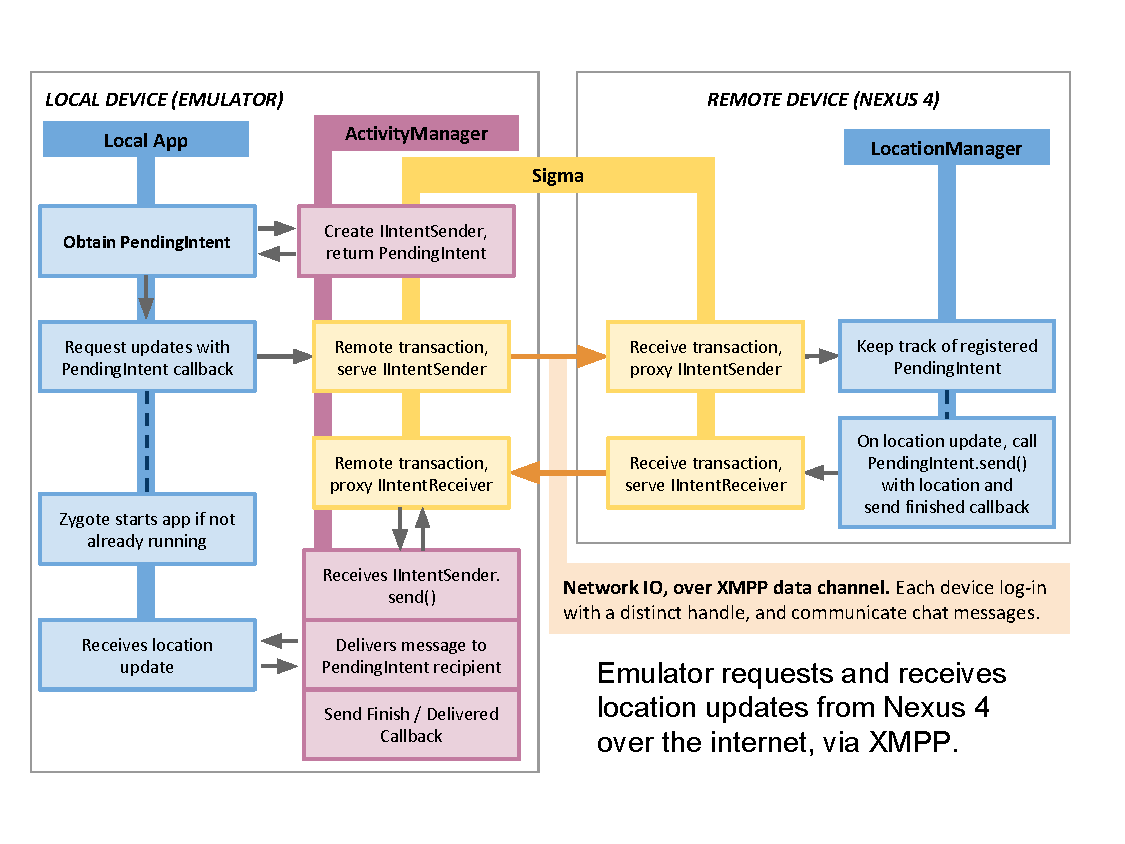
\includegraphics[width=\textwidth]{drawings/LocationPendingIntentExample.pdf}
\end{figure}

Useful metrics to measure include CPU load, memory usage, and network utilization on participating devices. Memory usage includes tracking heap allocation over time and also to track the number of native binder objects held by each device.

\textbf{TODO: Add plot showing memory and cpu usage. Point out the increasing number binder objects and sudden decrease. i.e. binder objects are dangling, then get garbage collected. one device sends a clean-up packet to the other so that Proxies are also cleaned up.}

\subsubsection{Remote Sensor Events}
The request to register for sensor events creates a SensorEventConnection which contains a BitTube object that is essentially an OO version of unix domain sockets. In establishing a SensorEventConnection, the file descriptor for the unix domain socket is communicated via binder. Subsequent communication of SensorEvents happens via this socket. We demonstrate that socket events are proxied and forwarded by Sigma. And plot the time difference between the native sensorevent callback and the remotely-routed sensorevent callback. Of course, the data channel used will have an impact on delay, and so we plot three different versions, each with progressively more latency and jitter.

\textbf{TODO: Add profiler results showing where the delay comes from... i.e. it is from the inefficient thread management in the HTTP server. There are ~30 SensorEvents per second, and this QPS is not handled elegantly by the server.}

\begin{figure}[h]
\centering
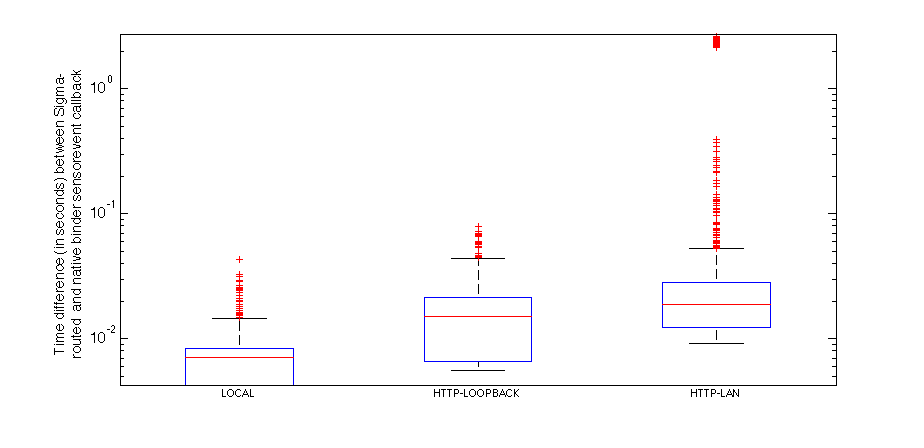
\includegraphics[width=0.7\textwidth]{plots/sensorevent_delay.png}
\end{figure}

Because there is jitter in received sensor events, it is necessary to depend on the timestamp provided by the sensorevent and not the timestamp of when the event is received by the listener callback. Also, depending on network conditions, it may not be possible to send sensor events at the full rate. Below we have simulated a limited bandwidth situation by routing HTTP packtes through a rate limited proxy. We see that as packets start to get queued, the latency increases to a point where packets are dropped or never make it back to the device.

\begin{figure}[h]
\centering
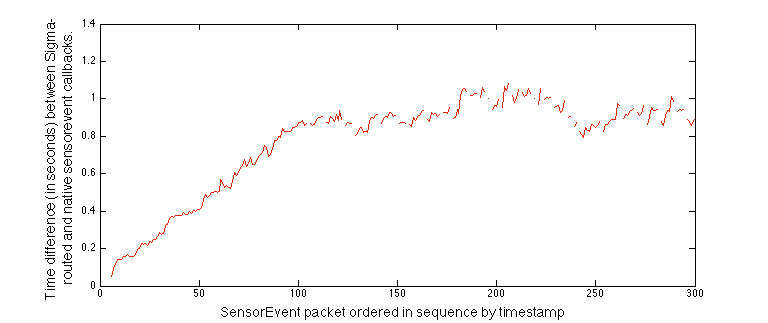
\includegraphics[width=0.7\textwidth]{plots/limited_bandwidth_increasing_latency.png}
\end{figure}

\section{Picture Sharing: An Example Distributed Applications purely in Android Binder}
\label{sec:ExampleApplication}

\begin{figure}[h]
\centering
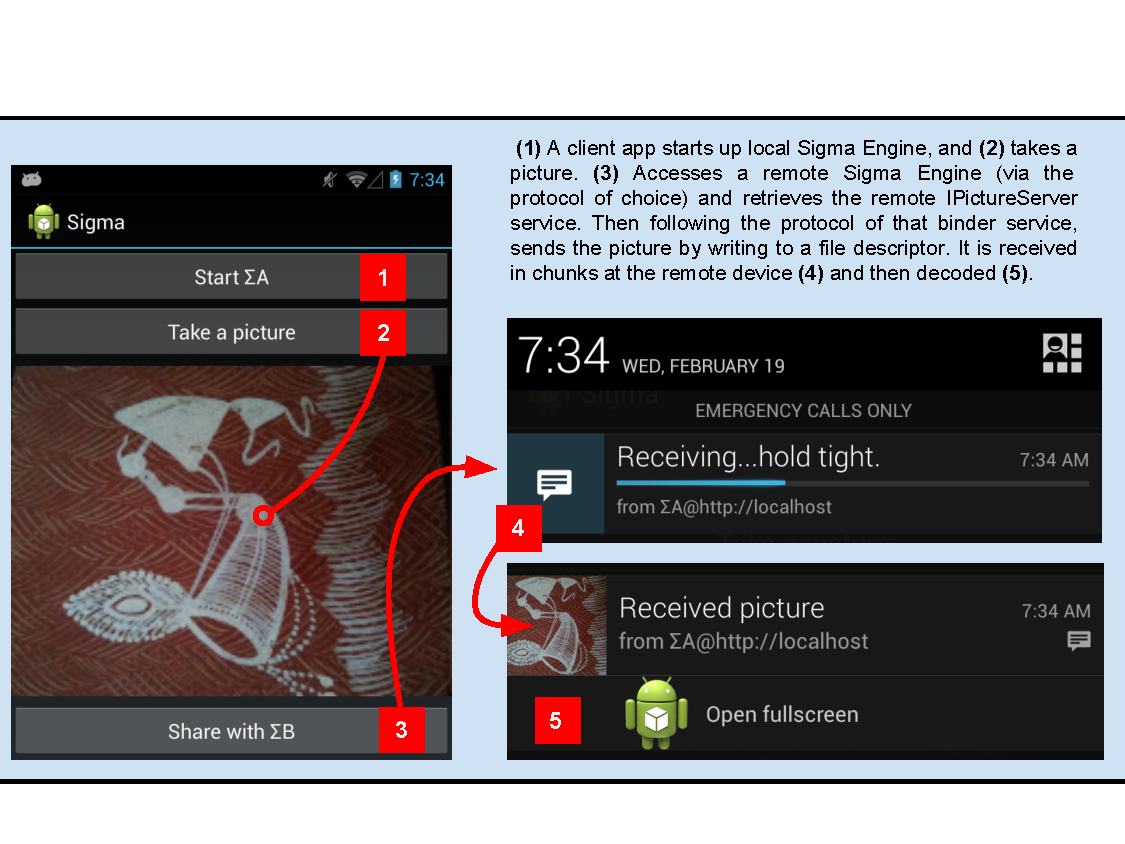
\includegraphics[width=\textwidth]{drawings/PictureChatExample.pdf}
\end{figure}

\begin{snippet}
interface IPictureChatServer {
  // Returns a fileDescriptor to which caller writes picture data.
  // Server polls the fileDescriptor to locally receives picture.
  // Sigma takes care of proxying file descriptor over network.
  // Also returns (modifies) PictureEntry with metadata as a new id for picture
  // used for subsequent request to the server.
  ParcelFileDescriptor /* readFrom */ requestPicturePut(
    ISigmaManager caller, inout PictureEntry entry);

  // Client passes in fileDescriptor to which server will write picture data.
  PictureEntry requestPictureGet(
    ISigmaManager caller, String uuid, in ParcelFileDescriptor writeTo);
}

class PictureEntry implements Parcelable {
    String uuid, from;
    int numBytes;
}
\end{snippet}

The design involves a single Binder service that acts as a picture server, this service can run on each device. Clients connects to a remote picture server to upload (or share) a picture. The service interface could have been one that receives the picture as single large byte array. However, to make the implementation more interesting as a test, the PictureChatServer operates on put- and get- requests which operate on returned or passed-in file descriptors, respectively. Picture data is communicated from one end to the other by performing IO on these file descriptors

The PictureChatServer already (via native bidner) allows remote processes to connect to it to put or get pictures. With Sigma an app on a remote device can access the same PictureChatServer service. Thus, a picture sharing app can be implemented simply by writing a regular Android binder service and add make it into a distributed app with Sigma.

By requiring caller Sigma Engine to be passed itself in as an argument (i.e. the ``ISigmaManager caller'' argument), the PictureChatServer can invoke RPCs to get details about the caller device and credentials. Here in this example, we use it to get the name and protocol of the remote caller. In the future, we expect this is useful to authenticate and restrict callers.

\section{Discussion and next steps}
\label{sec:Discussion}
Sigma is not a finished product, nor is it the ultimate distributed communication mechanism. Rather it is a good starting point for experimentation with Binder as a distributed communication mechanism. There are still some deficiencies that need to be fixed up, and important features of Binder remain unimplemented.

\subsubsection{Sigma as it is implemented today is not compatible with standard Android}
We have implemented Sigma as an Android APK that can be installed on all devices. First issue: much of the internal Java Android Runtime is hidden in the SDK, but fortunately is accessible to applications by employing reflection. Many features of Sigma are implemented this way, but is unsupported and not a stable API. For instance, here's how we retrieve the internal ServiceManager from Java.

\begin{snippet}
IBinder binder = sigma.getServiceManager(remoteURI);
Object serviceManager = Class.forName("android.os.ServiceManagerNative")
                    .getMethod("asInterface", IBinder.class)
                    .invoke(null, binder);
\end{snippet}

The second and larger issue is: the OO Binder implementation encapsulates the internal structures that we need to access to correctly manage binder messages. For this we had to minimally modify the Android Runtime, and so Sigma is not compatible with regular Android Runtimes running on devices today--i.e. without resorting to extreme hacks (like poking into memory addresses~\cite{FacebookDalvikHacks}) to get at the same data. The necessary modifications were covered in section~\ref{sec:AndroidRuntimeModifications}

\subsubsection{System services not portable across Android versions}
The RPC interface for the vast majority of system services is generated by the AIDL compiler--few like ServiceManager are hand-made. The generated RPC interfaces is not set in stone, it can vary with the different versions of the AIDL compiler or modifications to the AIDL source (like when switching the order of methods). For instance, a method foo() may be assigned code=1 in one version, and code=2 in another. Naturally, when operating between devices, identical RPC interfaces are expected by both ends. Generated AIDL interfaces do not have a notion of ``versions'' and it is impossible to tell from the Binder level whether two implementations of an interface (that go by the same name) have compatible internally generated structure. In testing, we have used the same version of Android among devices, compiled from the same source. So this issue was circumvented.

This limitation does not apply to RPC interfaces generated by third-party developers since they can fix a generated interface, ensuring backwards compatibility with previous versions by modifying the interface subsequently by hand.

\subsubsection{Parcels not portable between architectures}
Parcels were never implemented with the idea of portability. As we know, Parcels can contain binder objects and file descriptors which are obviously non-portable. Of course, the major implementation work in Sigma involved the managing of such objects, and provide a proxy for operating on them.

There is yet another aspect of Parcels that is non-portable, and this because primitive elemts are represented in a long byte array, copied byte-for-byte. This operations happens preserves endianness, and this fact is troublesome since a remote device of the the opposite endianness would incorrectly process primitive data elements when it comes time to read each element out of the parcel. Although this is a seemingly major obstacle to the use of binder as a distributed communication mechanism, in practice we see that most all Android devices are ARM-based, and ARM chips are bi-endian (there is a little switch to toggle to specify the endianness). Android, by specification, is little-endian for all such ARM-based devices~\cite{ARMLittleEndian}.

There is a way to make parcels portable, but we leave that to future work. Parcels store offsets to objects contained within, but not offsets to other types of primite data. We would first have to implement that feature (which will come with additional overhead in space requirements). To send over parcels, we would need to interpret each primitive element written into data array (is it an integer or a string of some length or something else?), marshalling each element in the Parcel separately using a canonical choice for endianness. Then on the other side, unmarshalling back into the data array would need to follow an analogous reverse procedure, decoding each element into the endianness appropriate for that system.

\subsubsection{XMPP and HTTP are not entirely satisfactory as data channels}
HTTP is only suitable over the local network since a HTTP server running on a device behind NAT is not accessible by others without additional configuration. XMPP uses a central chat server (accessible to all other devices) as a middleman. Having such a middleman incurs a performance penalty, and possible privacy concerns.

There are new technologies such as WebRTC~\cite{GoogleTalkLibrary} that seek to establish fully peer-to-peer connections. A signalling channel such as XMPP is used first to exchange descriptors between devices, and then a central server (typically hosted publically by a third-party) is involved in establishing a direct peer-to-peer connection. All subsequent communication is done via this connection. This same technology is used by Google Talk, and is soon going to become a w3c standard. Implementing and evaluating binder over network using webrtc data channels is left for future work.

\subsubsection{What happens when a remote binder dies? Or if the network channel disconencts?}
Binder supports via ``linkToDeath()'' the registering of callback that is invoked when the process hosting a remote binder unexpectedly dies. This is fortunate because we can use the same mechanism to notify of clients of a Sigma-managed Proxy Binder when networks disconnects. A ``linkToDeath'' is not mandatory for clients to use. Another feature of Android Binder is that a DeadObjectException is thrown when a RPC is invoked against a dead remote binder object. However, these two feature are not currently implemented in the prototype.

A final feature supported by Java Binder is handling exceptions that happen remotely. For instance, during a binder transaction an exception can be thrown by the remote process. This exception is written into the reply Parcel instead of the expected reply. Back at the Proxy, reading an exception throws an RemoteException. Since this is mechanism implemented through Binder messages exclusively, Sigma automatically supports such exception handling.

\subsubsection{Sigma disregards Android permissions model}
\label{sec:DealingWithAndroidPermissions}
Each Android app belongs to a distinct java package--this is the permissions namespace of the app. The PackageManager keeps track of the set of permissions that are requested by the package and also holds a map of the user-id assigned to each active package. Android activities and services within a package run as one or more processes which share the same user-id.

System services typically run as the root user. When an app (the caller) uses Binder IPC to make a call to another process like a system service, the callee can look up the process-id and user-id of the caller. This facility is baked into the BKM which is the component that handles the context switch from the caller to the callee (i.e. the caller thread sleeps, and wakes up a receiving thread in the callee's process). The callee can figure out (with the help of PackageManager) whether the caller has permission to access that particular system service. The system service in this way can reject unauthorized calls. This is a runtime security feature provided by BKM.

When the caller happens to be a process on a remote device, the Android security model breaks down. As implemented now, binder services are accessed and bound to the Sigma Engine, and not the process on the local device. The latter option does not make sense anyway since the remote ActivityManager does not know about the local process. Right now, Android permissions are effectively circumvented by having the Sigma Engine declaring all permissions--i.e. it essentially runs with root permissions. Any security is implemented separately by the Sigma Engine. And the permissions declared by the local process do not come into play.

There are obvious concerns with running with full permissions. One idea would be the remote device to communicate with the PackageManager on the local device, and grant an app all the permissions it is granted on the local device. However, this solution does not seem entirely satisfactory. Imagine an application requesting permission to access location of the local (its own) device means that it can also access location on all other remote devices.

It makes more sense for an app to be given permission to use a set of local services, and then a separate set of permissions granted to use remote services. For instance, a configuration panel on the remote device, much like a firewall, can be used to allow other devices access to certain services. Whenever the PackageManager is tasked with checking permissions for a binder object owned by Sigma Engine, such requests are redirected to Sigma. The implementation of such a panel and the necessary modifications to PackageManager is left for future work.

\subsection{Next Steps}
\label{sec:NextSteps}
In the long-term, it would be interesting to tightly couple two devices merging their Android Runtime state. Imagine that the local and remote PackageManager merge and present each device's components in their own namespace--one local, the other remote. Permissions to access services would have to be specified with the idea of a local and remote namespace as well. Consider also that the ActivityManager is merged. Sigma Engine would run within the runtime as part of the ActivityManager rather than as a separate package. With such tight coupling established, local components are able to connect to remote components directly through the ActivityManager's bindService(), the only difference is that apps specify a "remote" or "local" namespace to connect with. Tight coupling also solves some issues with notifications of binder service death. Lifecycle events of Android components on one device would automatically notify the other device, etc.

\bibliography{sigma}

\section{Appendix}

\subsection{Links to source code, available online}
\label{app:SourceCode}

\subsubsection{Sigma Engine and patched dependencies}
The main Sigma Engine that can be compiled into an Android package (or APK) can be found online.

\noindent~The root Sigma project with dependencies: \verb|https://github.com/kastur/SigmaRoot|.

\noindent~Or, without the dependencies at: \verb|https://github.com/kastur/Sigma|.

\noindent~The XMPP library is patched slightly, and is online: \verb|https://github.com/kastur/ASmack|

The code has been tested on a modified Android Runtime with a Android base version 4.2.2\_r1 on the Android Emulator and Nexus 4 device.
Modifications to the Android Runtime. Of course, the Sigma Android package will not function on a regular Android device. We have modified the Android 4.2.2\_r1 version source tree to support some features.

The modified runtime can be compiled and flashed on a real device or run on the emulator by following the directions at \verb|https://source.android.com/|. The following patches have to be applied to 2 modified sub-projects. The modified source tree for 2 sub-projects is available online:
\begin{Verbatim}
https://github.com/6b72/platform_frameworks_base/tree/sigma
https://github.com/6b72/platform_frameworks_native/tree/sigma
\end{Verbatim}

\noindent~The same modifications can be viewed as a patch to the baseline 4.2.2\_r1 version.
\begin{Verbatim}
https://github.com/6b72/platform_frameworks_base/compare/
763ef60466ac752a3031719fb86b08486c9946b1...3ae311d29691b3060e67bae1c891fb8fbbc1be0f

https://github.com/6b72/platform_frameworks_native/compare/
529cb9ed9c5d62d5b270cdd650380ae116382143...994ae7fa16165b3e85553d154111df0a2f5a5af3
\end{Verbatim}

\subsection{The Binder Kernel Module's binder\_call and handler function}
\label{app:binder_call}

\begin{snippet}
binder_call(binder_state *bs, binder_io *msg, binder_io *reply, void *target, int code)

bs -     each binder transaction and service gets its own state. Essentially contains
         a file descriptor to the binder kernel module.

msg -    essentially contains a data array with the following:
         * "android.os.IServiceManager" - name of the interface published in
                                          target binder service.
          * "com.example.service"        - name of the service to be  published
          * binder_service               - reference to the local binder service

reply -   contains the returned data array after the transaction. Can be null if there
          is no return value or we don't care about it.

target -  is a reference to a remote binder service already published. Usually
          references are obtained by a binder_call to the ServiceManager to retrieve
          published services. However, we can always make a binder call to the
          ServiceManager itself, which is always at the address (void*)0.

code -    is a non-specific value passed to the handler of the remote binder object.
          In this case, we pass an integer representing the action to be performed,
          where SVC_MGR_ADD_SERVICE is an pre-defined int.
\end{snippet}

All operations of a binder\_service are implemented inside of a handler function; the function signature resembles that of binder\_call:

\begin{snippet}
service_handler(binder_state *bs, binder_txn *txn,  binder_io *msg, binder_io *reply)
bs -      The initiating transaction.
txn -     essentially contains code (from binder_call), and the calling uid and pid.
msg -     The incoming message from binder_call.
reply -   The return value should be written out here, if any
\end{snippet}

\subsection{The flat\_binder\_object struct}
This struct holds either a local pointer to a binder service or a kernel-module provided handle. This same struct is used for storing file descriptors as well.

\begin{snippet}
struct flat_binder_object {
  unsigned long type, flags  /* header */
  union {
    void *binder;        /* local object */
    signed long handle;  /* remote object */
  };
  void *cookie;          /* extra data */
};
\end{snippet}

\subsection{The binder\_io struct}
This struct holds the data for binder transactions as byte arrays. Objects and file descriptors are flattened as flat\_binder\_object structs and written into the data array, with the offset for each object written stored in the offs array.

The Java and C++ binder transactions operate on Parcel objects which encapsulate a binder\_io data structure.

\begin{snippet}
struct binder_io {
  char *data;            /* start of data buffer */
  uint32_t *offs;        /* array of offsets */
  uint32_t data_avail;   /* bytes available in data buffer */
  uint32_t offs_avail;   /* entries available in offsets array */
};
\end{snippet}

\subsection{IServiceManager's object-oriented service interface}
\label{app:ServiceManager}

\begin{snippet}
class IServiceManager : public IInterface {
 public:
    // Retrieve an existing service, blocking for a few seconds if it doesn't yet exist.
  virtual sp<IBinder> getService(const String16& name) const = 0;
    // Retrieve an existing service, non-blocking.
  virtual sp<IBinder> checkService(const String16& name) const = 0;
    // Register a service.
  virtual status_t addService(const String16& name, const sp<IBinder>& service, ..) = 0;
    // Return list of all existing services.
  virtual Vector<String16> listServices() = 0;
}
\end{snippet}

Note that what is not captured by the interface definition alone is that arbitrary process do not have permission to add new services. Inside the invokation of addService is a call to getCallingUid(), which is used to enforce permissions, limiting it so that only system processes may add services.

getCallingUid() and getCallingPid() are features of the Binder Kernel Module to get information about the caller process.


\subsection{Examples of Sigma (Wire) messages}
\label{app:WireExchange}
The following set of figures show in detail the Wire messages exchanged between two Sigma Engines (implemented via a LOCAL protocol, with engines running on same device and communicating to each other via native binder). The messages correspond to the example from the beginning of "Design of Sigma" section, where a remote Sigma Engine reference is first retrieved via RPC to a local Sigma Engine, and then a reference to remote service is obtained.
\begin{figure}[h!]
\centering
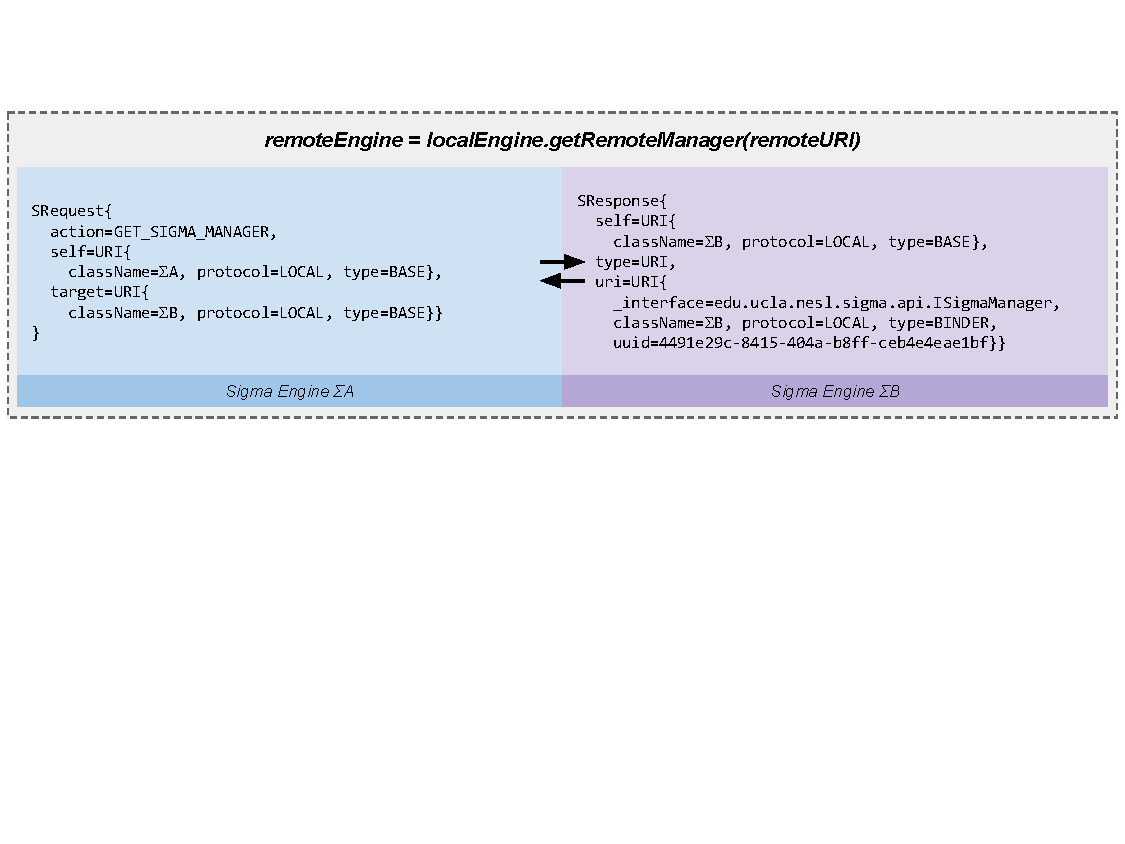
\includegraphics[width=\textwidth]{drawings/WireExchange1.pdf}
\end{figure}
\begin{figure}[h!]
\centering
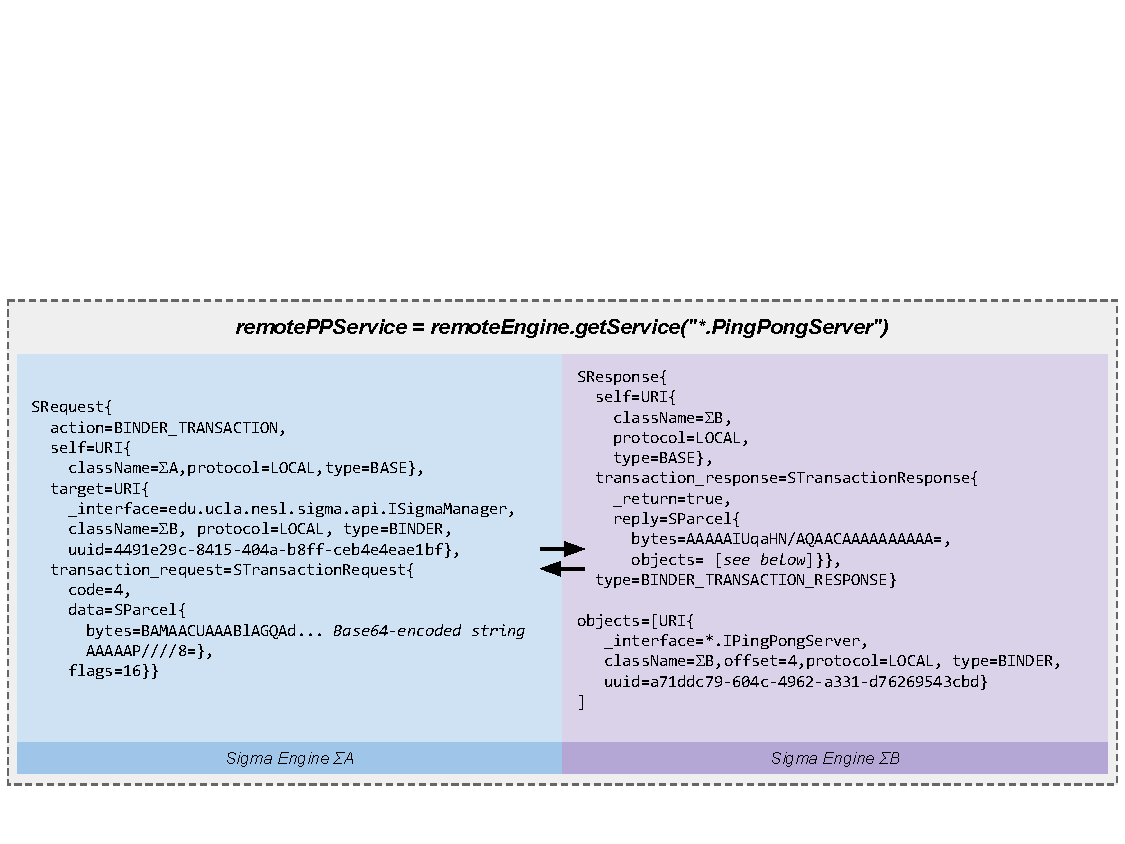
\includegraphics[width=\textwidth]{drawings/WireExchange2.pdf}
\end{figure}

Here, since we are operating under the LOCAL protocol, all transactions proxy binder objects are transit through the local Sigma Engine and then to the remote Sigma Engine (which also runs on the same device as a different process), and then from there to the native binder service. Naturally this the transit from local to remote Sigma Engine will take over the network (through HTTP or XMPP) for those implementations.

\subsection{Wire messages exchanged during a recursive binder RPC}
\label{app:WireExchangeRecursive}
An exchange of Wire messages detailing a recursive binder that take place between two Sigma Engine instances from the example of the PingPong service.
\begin{figure}[h!]
\centering
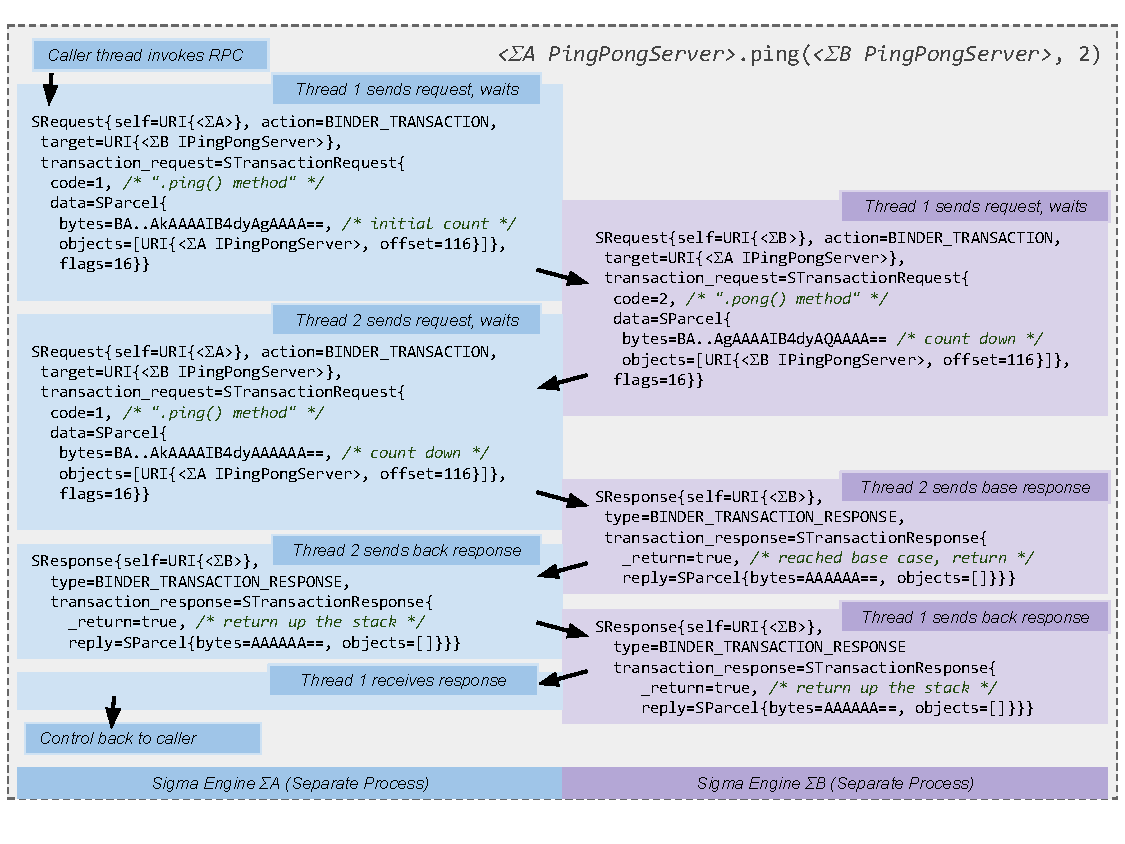
\includegraphics[width=\textwidth]{drawings/WireExchangeRecursive.pdf}
\end{figure}

\end{document}
